% Options for packages loaded elsewhere
\PassOptionsToPackage{unicode}{hyperref}
\PassOptionsToPackage{hyphens}{url}
%
\documentclass[
]{book}
\usepackage{lmodern}
\usepackage{amsmath}
\usepackage{ifxetex,ifluatex}
\ifnum 0\ifxetex 1\fi\ifluatex 1\fi=0 % if pdftex
  \usepackage[T1]{fontenc}
  \usepackage[utf8]{inputenc}
  \usepackage{textcomp} % provide euro and other symbols
  \usepackage{amssymb}
\else % if luatex or xetex
  \usepackage{unicode-math}
  \defaultfontfeatures{Scale=MatchLowercase}
  \defaultfontfeatures[\rmfamily]{Ligatures=TeX,Scale=1}
\fi
% Use upquote if available, for straight quotes in verbatim environments
\IfFileExists{upquote.sty}{\usepackage{upquote}}{}
\IfFileExists{microtype.sty}{% use microtype if available
  \usepackage[]{microtype}
  \UseMicrotypeSet[protrusion]{basicmath} % disable protrusion for tt fonts
}{}
\makeatletter
\@ifundefined{KOMAClassName}{% if non-KOMA class
  \IfFileExists{parskip.sty}{%
    \usepackage{parskip}
  }{% else
    \setlength{\parindent}{0pt}
    \setlength{\parskip}{6pt plus 2pt minus 1pt}}
}{% if KOMA class
  \KOMAoptions{parskip=half}}
\makeatother
\usepackage{xcolor}
\IfFileExists{xurl.sty}{\usepackage{xurl}}{} % add URL line breaks if available
\IfFileExists{bookmark.sty}{\usepackage{bookmark}}{\usepackage{hyperref}}
\hypersetup{
  pdftitle={Communication Theories},
  pdfauthor={Mike Nguyen},
  hidelinks,
  pdfcreator={LaTeX via pandoc}}
\urlstyle{same} % disable monospaced font for URLs
\usepackage{color}
\usepackage{fancyvrb}
\newcommand{\VerbBar}{|}
\newcommand{\VERB}{\Verb[commandchars=\\\{\}]}
\DefineVerbatimEnvironment{Highlighting}{Verbatim}{commandchars=\\\{\}}
% Add ',fontsize=\small' for more characters per line
\usepackage{framed}
\definecolor{shadecolor}{RGB}{248,248,248}
\newenvironment{Shaded}{\begin{snugshade}}{\end{snugshade}}
\newcommand{\AlertTok}[1]{\textcolor[rgb]{0.94,0.16,0.16}{#1}}
\newcommand{\AnnotationTok}[1]{\textcolor[rgb]{0.56,0.35,0.01}{\textbf{\textit{#1}}}}
\newcommand{\AttributeTok}[1]{\textcolor[rgb]{0.77,0.63,0.00}{#1}}
\newcommand{\BaseNTok}[1]{\textcolor[rgb]{0.00,0.00,0.81}{#1}}
\newcommand{\BuiltInTok}[1]{#1}
\newcommand{\CharTok}[1]{\textcolor[rgb]{0.31,0.60,0.02}{#1}}
\newcommand{\CommentTok}[1]{\textcolor[rgb]{0.56,0.35,0.01}{\textit{#1}}}
\newcommand{\CommentVarTok}[1]{\textcolor[rgb]{0.56,0.35,0.01}{\textbf{\textit{#1}}}}
\newcommand{\ConstantTok}[1]{\textcolor[rgb]{0.00,0.00,0.00}{#1}}
\newcommand{\ControlFlowTok}[1]{\textcolor[rgb]{0.13,0.29,0.53}{\textbf{#1}}}
\newcommand{\DataTypeTok}[1]{\textcolor[rgb]{0.13,0.29,0.53}{#1}}
\newcommand{\DecValTok}[1]{\textcolor[rgb]{0.00,0.00,0.81}{#1}}
\newcommand{\DocumentationTok}[1]{\textcolor[rgb]{0.56,0.35,0.01}{\textbf{\textit{#1}}}}
\newcommand{\ErrorTok}[1]{\textcolor[rgb]{0.64,0.00,0.00}{\textbf{#1}}}
\newcommand{\ExtensionTok}[1]{#1}
\newcommand{\FloatTok}[1]{\textcolor[rgb]{0.00,0.00,0.81}{#1}}
\newcommand{\FunctionTok}[1]{\textcolor[rgb]{0.00,0.00,0.00}{#1}}
\newcommand{\ImportTok}[1]{#1}
\newcommand{\InformationTok}[1]{\textcolor[rgb]{0.56,0.35,0.01}{\textbf{\textit{#1}}}}
\newcommand{\KeywordTok}[1]{\textcolor[rgb]{0.13,0.29,0.53}{\textbf{#1}}}
\newcommand{\NormalTok}[1]{#1}
\newcommand{\OperatorTok}[1]{\textcolor[rgb]{0.81,0.36,0.00}{\textbf{#1}}}
\newcommand{\OtherTok}[1]{\textcolor[rgb]{0.56,0.35,0.01}{#1}}
\newcommand{\PreprocessorTok}[1]{\textcolor[rgb]{0.56,0.35,0.01}{\textit{#1}}}
\newcommand{\RegionMarkerTok}[1]{#1}
\newcommand{\SpecialCharTok}[1]{\textcolor[rgb]{0.00,0.00,0.00}{#1}}
\newcommand{\SpecialStringTok}[1]{\textcolor[rgb]{0.31,0.60,0.02}{#1}}
\newcommand{\StringTok}[1]{\textcolor[rgb]{0.31,0.60,0.02}{#1}}
\newcommand{\VariableTok}[1]{\textcolor[rgb]{0.00,0.00,0.00}{#1}}
\newcommand{\VerbatimStringTok}[1]{\textcolor[rgb]{0.31,0.60,0.02}{#1}}
\newcommand{\WarningTok}[1]{\textcolor[rgb]{0.56,0.35,0.01}{\textbf{\textit{#1}}}}
\usepackage{longtable,booktabs}
\usepackage{calc} % for calculating minipage widths
% Correct order of tables after \paragraph or \subparagraph
\usepackage{etoolbox}
\makeatletter
\patchcmd\longtable{\par}{\if@noskipsec\mbox{}\fi\par}{}{}
\makeatother
% Allow footnotes in longtable head/foot
\IfFileExists{footnotehyper.sty}{\usepackage{footnotehyper}}{\usepackage{footnote}}
\makesavenoteenv{longtable}
\usepackage{graphicx}
\makeatletter
\def\maxwidth{\ifdim\Gin@nat@width>\linewidth\linewidth\else\Gin@nat@width\fi}
\def\maxheight{\ifdim\Gin@nat@height>\textheight\textheight\else\Gin@nat@height\fi}
\makeatother
% Scale images if necessary, so that they will not overflow the page
% margins by default, and it is still possible to overwrite the defaults
% using explicit options in \includegraphics[width, height, ...]{}
\setkeys{Gin}{width=\maxwidth,height=\maxheight,keepaspectratio}
% Set default figure placement to htbp
\makeatletter
\def\fps@figure{htbp}
\makeatother
\setlength{\emergencystretch}{3em} % prevent overfull lines
\providecommand{\tightlist}{%
  \setlength{\itemsep}{0pt}\setlength{\parskip}{0pt}}
\setcounter{secnumdepth}{5}
\usepackage{booktabs}
\ifluatex
  \usepackage{selnolig}  % disable illegal ligatures
\fi
\usepackage[]{natbib}
\bibliographystyle{apalike}

\title{Communication Theories}
\author{Mike Nguyen}
\date{2021-04-07}

\begin{document}
\maketitle

{
\setcounter{tocdepth}{1}
\tableofcontents
}
\hypertarget{prerequisites}{%
\chapter{Prerequisites}\label{prerequisites}}

This book is based on the two communications seminars

\begin{longtable}[]{@{}cc@{}}
\toprule
Course & Professor\tabularnewline
\midrule
\endhead
Interpersonal Communication & Haley Horstman\tabularnewline
Organizational Communication & Debbie Dougherty\tabularnewline
\bottomrule
\end{longtable}

Communication is defined as the exchange of messages.

\begin{Shaded}
\begin{Highlighting}[]
\FunctionTok{install.packages}\NormalTok{(}\StringTok{"bookdown"}\NormalTok{)}
\CommentTok{\# or the development version}
\CommentTok{\# devtools::install\_github("rstudio/bookdown")}
\end{Highlighting}
\end{Shaded}

\hypertarget{part-interpersonal}{%
\part{INTERPERSONAL}\label{part-interpersonal}}

\hypertarget{intro}{%
\chapter{Introduction}\label{intro}}

History

\begin{itemize}
\tightlist
\item
  Cornell School: study of speech from a humanities perspective
\item
  Midwestern School: study speech as a science
\end{itemize}

According to \citep{Baxter_2008}, interpersonal communication is ``the
production and processing of verbal and nonverbal messages between two
or a few persons''.

Three perspectives to study interpersonal communication \citep{Baxter_2008}

\begin{itemize}
\tightlist
\item
  \protect\hyperlink{individually-centered}{Individually Centered}
\item
  \protect\hyperlink{interactiondiscourse-centered}{Interaction/discourse Centered}
\item
  \protect\hyperlink{relationship-centered}{Relationship Centered}
\end{itemize}

Theory and data should be an interactive process. We should understand
the conceptual boundaries of a theory, we should not apply it
everywhere, generously improve it or dismiss it. Usually, there aren't
one ultimate theory that has its own sovereignty \citep{Higgins_2004}. Each
theory has its own assumptions. ``Making different predictions is not hte
same as making competing predictions''. \citep{Higgins_2004}. a phenomenon can
be explained by multiple theories, with different reasons, which shows
its robustness.

A theory must be:

\begin{enumerate}
\def\labelenumi{\arabic{enumi}.}
\tightlist
\item
  Testable
\item
  Coherent
\item
  Economical/Parsimonious
\item
  Generalizable
\item
  Explanability
\end{enumerate}

A theory is like a child. Developing a theory is like parenting.

\begin{itemize}
\tightlist
\item
  Don't abuse
\item
  Don't spoil
\item
  Knowing your theory and its limitation.
\end{itemize}

\citep[pp.~5-30]{miller1995} Assumption of interpersonal communication: "
when people communicate, they make predictions about the effects, or
outcomes, of their communication behavior". Prediction can be made
consciously or unconsciously; hence, communication has creative element.
Two sets of factors influence prediction:

\begin{itemize}
\tightlist
\item
  \textbf{situational} set: ``the given, unalterable features of a
  communication setting''.\\
\item
  \textbf{dispositional} set: ``our past experience and our future
  expectations dispose us to look for certain behaviors and to
  interpret them in certain ways''.
\end{itemize}

Levels of analysis used in making prediction

\begin{enumerate}
\def\labelenumi{\arabic{enumi}.}
\item
  Cultural:

  \begin{itemize}
  \tightlist
  \item
    culture is ``the sum of characteristics, beliefs, habits,
    practices, and language shared by a large group of people,''. +
    can be either heterogeneous or homogeneous (homogeneity
    increases prediction accuracy).
  \item
    norm is ``a recurrent, observable pattern'', which help predict
    behavior
  \item
    ideology also helps predict responses to certain messages.
  \item
    prediction based on cultural data can be erroneous. The more
    culturally diverse a society is, the more error that you will
    make.
  \end{itemize}
\item
  Sociological:

  \begin{itemize}
  \tightlist
  \item
    A membership group is ``a class of people who share certain
    common, characteristics, either by their own volition or because
    of some criteria imposed by the predictor''.
  \end{itemize}
\item
  Psychological

  \begin{itemize}
  \tightlist
  \item
    Sources of behavioral differences: - learning experiences
  \item
    reactions to experiences
  \item
    perception by observers of behavior.
  \end{itemize}
\end{enumerate}

``Generally know a little about a great number of people and a lot about
very few people''

\[
\text{Generalization}  \\
\text{Cultural} \\
\downarrow \\
\text{Sociological} \\
\downarrow \\
\text{Psychological} 
\]

``When predictions about communication outcomes are based primarily on a
cultural or sociological level of analysis, the communicators are
engaged in non-interpersonal communication; when predictions are based
primarily on a psychological level of analysis, the communicators are
engaged in interpersonal communication''.

Cultural and sociological = non-interpersonal communication\\
Psychological = interpersonal communication.

Stimulus generalization (may have more predictive errors) vs.~stimulus
discrimination.

\begin{itemize}
\item
  We make stimulus generalization initially because it is not feasible
  to base our prediction on psychological data.
\item
  very little interpersonal communication in our society:

  \begin{itemize}
  \tightlist
  \item
    teleological view: we should strive for interpersonal level
  \item
    pragmatic view: we don't need to get to the interpersonal level
  \end{itemize}
\item
  not every communicate interpersonally in similar ways.
\item
  the difference between interpersonal communication and interpersonal
  relationships is that in interpersonal relationship, two people must
  be communicating interpersonally
\end{itemize}

\citep{wilmot1995}

There are two growth trajectories for love relationships:

\begin{itemize}
\tightlist
\item
  whirlwind
\item
  friendship
\end{itemize}

The interpenetration of communication and relationships

\begin{itemize}
\item
  Principle 1: Relational Definition emerge from recurring episodic
  enactments.

  \begin{itemize}
  \tightlist
  \item
    An episode is ``a nonverbal and verbal communication event''.
  \item
    relational translation: attach relationship meaning to the
    episodes.
  \item
    ``the more frequently a relational definition is reinforced by
    episodic enactments, the more potent it becomes''.
  \end{itemize}
\item
  Principle 2: Relationship Definitions ``Frame'' or Contextualize
  Communication Behavior

  \begin{itemize}
  \tightlist
  \item
    ``the meaning of our communication behaviors is dependent on the
    relational frame where they occur''.\\
  \item
    ``communication is interpreted and associated within given
    relational definitions''.
  \end{itemize}
\item
  Principle 3: Relationship types are not necessarily mutually
  exclusive
\item
  Principle 4: relationship Definition and communication episodes
  reciprocally frame one another
\end{itemize}

\textbf{A Theory of Embeddedness}

\begin{itemize}
\item
  Relationship Constellations

  \begin{itemize}
  \tightlist
  \item
    definition: ``interconnected networks that form patterns''.
  \item
    the constellations influences initiating relationships by:
  \item
    the network we are in
  \item
    social norms
  \item
    the postilion of initiator and potential partner in the network
  \item
    direct action, or approval/disapproval by others in the network
    on your choice.
  \item
    density of the network also influences the overall
    constellation.
  \item
    not only actual actions by the constellation members that affect
    you, even your anticipation of the reaction of those members
    also affects you. \citep{Surra_1990} + people are influenced by the
    support or disapproval of the network
  \item
    ``Romeo and Juliet effect'': disapproval of parents strengthens
    relationship's bonds.
  \end{itemize}
\item
  Cultural Considerations
\end{itemize}

\textbf{Self and Other in relation}

\begin{itemize}
\tightlist
\item
  Self was defined as independent and autonomous.(e.g., in psychology
  mostly dysfunctionality exists mainly in self )
\end{itemize}

\textbf{Paradigm 1: The Individual Self}

Self and Others are ``independent units that are connected by the
relational thread.'' Or mere overlap of the two separate autonomous
selves who just happen to have enough in common to create a
relationship."

Relationship difficulties are identified by the degree of blame of the
other.

Social exchange model (assume that we try to maximize profit in
relationships ). Hence, we focus on building self (self-satisfaction),
not relationship.

Postmodern thinking:

Constructedness: see ``people as forming and reforming their selves
within each relationship''.

\textbf{relational self}

\textbf{Paradigm 2: The Embedded Self}

``The identity of''I" is possible solely through the identity of the
other who recognizes me, and who in turn is dependent upon my
recognition". (Wilber, 1932, p.272)

\textbf{The Dialectical Perspective}\\
There is a dynamic interplay between opposites that we need to look at.
Everything is interdependent. trade off between exactitude of factual
language and seeing things in a totality way.\\
External (e.g., contradiction between autonomy and integration, me vs.
we, independence vs.~interdependence, or expressiveness vs.
protectiveness) and internal dialectical tensions in relationships

\textbf{Paradigm 3: Nonseparable self/other/relationship}

the self is the result of interaction with others.

Communication is ``a conjoint reality created by two people in relation
to each other''

Paradigm I \textbar{} communication is a static, linear, noninteractive event.

Transformation = Expression + Connection

\citep{Baxter_2004}

ground relational dialectics theory:

\begin{enumerate}
\def\labelenumi{\arabic{enumi}.}
\item
  Dialogue as constitutive process

  \begin{itemize}
  \tightlist
  \item
    ``Communication as a conduit through which a variety of
    antecedent psychological ans sociological factors are played
    out''.
  \item
    Alternative: ``Communication as constitutive'': communication
    constitutes persons and relationships.
  \item
    ``An individual knows self only from the outside, as he or she
    conceives others see him or her. The self, then, is invisible to
    itself and dependent for its existence on the other''. Hence,
    self is ``a fluid and dynamic relation between self and other''. +
    self-becoming resembles self-expansion model.
  \end{itemize}
\item
  Dialogue as dialectical flux

  \begin{itemize}
  \tightlist
  \item
    Dialogue is ``simultaneously unity and difference''. hence, social
    life is a dialogue ``constituted in the dialectical, or
    contradictory, interplay of centripetal and centrifugal forces''.
  \item
    contrast to Hegelian approach to dialogue
  \end{itemize}
\item
  Dialogue as aesthetic moment
\item
  Dialogue as utterance
\item
  Dialogue as critical sensibility
\end{enumerate}

Braithwaite's Perspectives on interpersonal communication

\begin{itemize}
\tightlist
\item
  Numerical Perspective
\item
  Situational and contextual perspective
\item
  Developmental Perspective
\item
  Levels of Info Perspective \citep{miller1995}
\item
  Relational (Stewart) focusing on the content.
\item
  Constitutive Approach \citep{Baxter_2004}
\end{itemize}

Def of IPC = when predictions about comm outcomes are based primarily on
a psych level of analysis (p.~22)\\
IPC occurs when:\\
1. Predictions are based on personal level info\\
2. Have direct experience with other person\\
3. Initial interactions are rarely interpersonal\\
4. Most interactions are non-interpersonal\\
5. Relationships exist when both people are communicating
interpersonally

Chapter 2 (Stewart (2019))

Communication is ``the processes humans use to construct meaning
together''.

\begin{enumerate}
\def\labelenumi{\arabic{enumi}.}
\tightlist
\item
  Since humans live in worlds of meaning that are constantly
  constructed, none can affect the process significantly.
\item
  Culture figures (ethnicity, gender, age, social class, sexual
  orientation, etc) affect communication and how you respond to it.
\item
  we collaboratively build the sense of selves (i.e., identity) when
  engaging in communication.
\item
  Conversations are a tools for communication.
\item
  A useful skills in communicating is ``nexting''.
\end{enumerate}

Communication is ``the continuous, complex, collaborative, process of
verbal and nonverbal meaning-making through which we construct the
worlds of meaning we inhabit.''

Worlds of meanings:

\begin{itemize}
\tightlist
\item
  space
\item
  time
\item
  laws of physics
\item
  culture
\item
  relationships
\item
  work (for adults).
\end{itemize}

Interpersonal Communication:\\
``people involved are contacting each other as persons''

Characteristics that distinguish persons across cultures:

\begin{itemize}
\tightlist
\item
  uniqueness: noninterchangeability (either experiential or genetic)
\item
  unmeasurability: human can't be described by parts. even though
  cognitive scientists try to assign schematas or cognitive patters/
  Emotions and feeling are embedded in communications.
\item
  Responsiveness is different from reaction.
\item
  reflectiveness: being aware of what's around, but also aware of your
  own awareness.
\item
  addressability: difference between talking to and talking with
  (i.e., addressable). directed or aimed at.
\end{itemize}

``the term interpersonal labels the kind of communication that happens
when the people involved talk and listen in ways that maximize the
presence of the personal''.

\citep{Floyd_2014}

Interpersonal communication is defined as ``Any communication at the
intrapersonal, small group, public, or mass levels.''

Boundary condition includes:

\begin{itemize}
\tightlist
\item
  dyad relationships
\item
  ``IPC as close, supportive, relationship-maintaining communication
  occurring between people (whether in a dyad or not'')
\end{itemize}

\hypertarget{individually-centered}{%
\chapter{Individually Centered}\label{individually-centered}}

\hypertarget{uncertainty-management-theories}{%
\section{Uncertainty Management Theories}\label{uncertainty-management-theories}}

\hypertarget{problematic-integration-theory}{%
\subsection{Problematic Integration Theory}\label{problematic-integration-theory}}

Problematic Integration (PI) theory: From the theories of planned behavior and reasoned action, we believe that we can
predict people's behaviors because people are assumed to be ``rational''. However, there are communication substance that
could input uncertainty and inconsistency expectations to predict human behavior.

\begin{itemize}
\item
  Goals:

  \begin{itemize}
  \tightlist
  \item
    find important and ubiquitous communication process
  \item
    increase sophistication
  \item
    encourage other ways of understanding
  \item
    increase communicators' empathy and compassion.
  \end{itemize}
\item
  Forms of PI:

  \begin{itemize}
  \tightlist
  \item
    Uncertainty
  \item
    Diverging expectations and desires
  \item
    Ambivalence
  \item
    Impossible desires (theoretical vs.~practical impossibility).
  \end{itemize}
\item
  Discussion regarding PI can deepen or hurt relationships
\item
  Encounter PI, we can engage in presentational and avoidance rituals.
\item
  PI defines uncertainty as ``difficulty forming a mental association''. \citep{Babrow_2009}

  \begin{itemize}
  \tightlist
  \item
    form-specific adaptation of messages means ``communicating in ways that speak to the precise dilemma.''
    \citep{Babrow_2009}
  \end{itemize}
\end{itemize}

\hypertarget{uncertainty-management-theory}{%
\subsection{Uncertainty Management Theory}\label{uncertainty-management-theory}}

Uncertainty Management (UM)

\begin{itemize}
\item
  Based on two post-positivist sources:

  \begin{itemize}
  \tightlist
  \item
    Uncertainty reduction theory \citep{BERGER_1975}: managing uncertainty
  \item
    Cognitive theory of uncertainty in illness \citep{Mishel_1990}: depending on context, uncertainty can be either good
    or bad
  \end{itemize}
\item
  Uncertainty must be appraised.
\item
  Notion of management = control
\end{itemize}

Research and practical application (e.g., health, education, )\\
Evaluation: not achievable under post-positivist because of its blurry boundary conditions. But under interpretivist, it
can make more sense due to its contextual meanings.

Application:\\
Taking Control: The Efficacy and Durability of a Peer-Led Uncertainty Management Intervention for People Recently
Diagnosed With HIV \citep{Brashers_2016}: Uncertainty management need to be adaptable. Due to the changing nature of HIV
skills and information for patients need to be communicated continuously. Supported by the theories of social support,
uncertainty management can be facilitated with peer support. participant report less illness-related uncertainty,
greater access to social support, and more satisfaction with the social support compared to the control group. \textbf{Illness
uncertainty} was assessed with \citep{MISHEL_1981}.

Example

\citep{SHARABI_2017} Effects of the first FtF date on romantic relationship development:

\begin{itemize}
\tightlist
\item
  Relational choice models of romantic relationships: Choosing partners that make the most sense to you (fit an image
  of an ideal mates).
\item
  Disillusionment models of romantic relationship: When you see other's aspects (e.g., personality, behaviors) of your
  partner, you might no longer be interested in your partner.
\end{itemize}

Predicting first date success in online dating

\begin{itemize}
\tightlist
\item
  Similarity and uncertainty as predictors: users want to reduce uncertainty before meeting offline.\\
\item
  Communication as moderating role.
\end{itemize}

Interestingly, people disclose more deeply online compared to offline \citep{Tidwell_2002}

\hypertarget{theory-of-motivated-informaiton-management-tmim}{%
\subsection{Theory of Motivated Informaiton Management (TMIM)}\label{theory-of-motivated-informaiton-management-tmim}}

Born from the frustration with \protect\hyperlink{problematic-integration-theory}{Problematic Integration Theory}, \protect\hyperlink{uncertainty-management-theory}{Uncertainty Management Theory} interepretivist
orientation, and desire to incorporate individual experience's complexity with uncertainty and predictive specificity.

The theory has its basis on:

\begin{itemize}
\tightlist
\item
  Subjective Expected Utility theory \citep{Fischhoff_1983}\\
\item
  social Cognitive theory \citep{Locke_1987}
\item
  Theories of bounded rationality \citep{Kahneman_2003}: People make suboptimal choice due to other emotions and bias
  factors.
\end{itemize}

Due to its laborious process of decision, theory of motivated information management only applies to cases where the
person thinks a decision is sufficient important.

Phases:

\begin{itemize}
\item
  Interpretation Phase: recognize the difference (called \textbf{uncertainty discrepancy}) in desired uncertainty and
  current uncertainty, which mostly produces anxiety, but sometimes hope, anticipation, anger.\\
\item
  Evaluation Phase: :appraisal of uncertainty impacts assessments made in the evaluation phase", which makes you think
  about

  \begin{itemize}
  \item
    Outcome expectancy: what happen if you search for more info\\
  \item
    Efficacy: whether you are able to do the search.

    \begin{itemize}
    \tightlist
    \item
      Communication efficacy: whether a person has the skill to seek info.\\
    \item
      Target efficacy: whether the target of the info search actually has and would be willing to share it.\\
    \item
      Coping efficiency: whether a person could emotionally, relational, or financially deal with what he or she
      expects to learn.
    \end{itemize}
  \end{itemize}
\item
  Decision Phase: people are likely to seek info when they expect positive outcomes with high levels of efficacy.
\end{itemize}

\begin{center}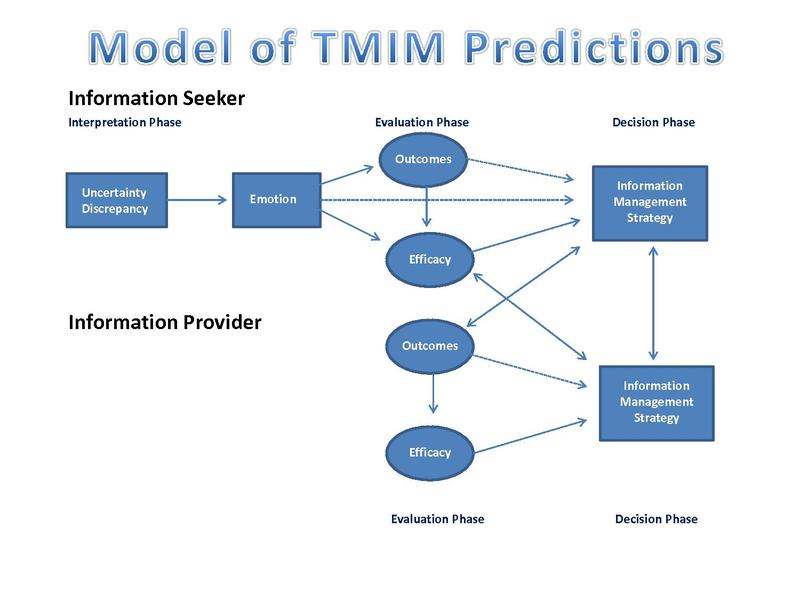
\includegraphics[width=11.11in]{images/Model of TMIM Predicitons} \end{center}

(picture from \citep{Baxter_2008})

Note: Information providers go through the same process with only the latter two phases (evaluation and decision).

Research and Practical Application: (e.g., education, health)

Evaluation:

\begin{itemize}
\item
  Benefits:

  \begin{itemize}
  \tightlist
  \item
    Draw attention to communication efficiency, and outcome expectancy
  \item
    Good theory: based on testability, heuristics, parsimony, scope condition
  \end{itemize}
\item
  Improvement:

  \begin{itemize}
  \tightlist
  \item
    may need to include efficacy's strength as mediator. Depending on the positivity or negativity of expectations.
    relationship between outcome expectancies and efficacy, and between outcome expectancies and information seeking
    may differ
  \end{itemize}
\end{itemize}

Example:

\citep{Morse_2013} social networks and information seeking influence drug use. From Social Cognitive Theory, and Cognitive
Developmental Theory, social norms and peer influence serve as bases for aversive behaviors to be accepted. According to
\citep{Wolfson_2000}, false consensus support can help explain students overestimate of the positive attitudes of their
social network supported by the fact that they are uncertain about their social network's opinions.

\hypertarget{attribution-theory}{%
\section{Attribution Theory}\label{attribution-theory}}

``how and why we try to answer''how and why" questions is referred to as attribution theory" \citep{Baxter_2008}

originated from psychology. ``The more important or unexpected the event, the more likely people are to seek an
explanation to make sense of that outcome. We make sense of such events primarily by determining what the cause is.''

Goals

\begin{itemize}
\tightlist
\item
  Event causation: understand actions or events by attributing cause(s) to behavior.
\item
  Trait inference: make inference about a person' characteristics that makes sense of that person's behavior.
\end{itemize}

Dimensions when making attributions:

\begin{itemize}
\tightlist
\item
  locus: interval or external to the person
\item
  Stability: temporary or enduring
\item
  Specificity: causes is unique or universal
\item
  Responsibility: the extent to which a person contribute to the event
\end{itemize}

Focus on:

\begin{itemize}
\item
  Correspondence: ``When attributions are informative of a person's nature or personality, they are considered
  \textbf{"correspondent"} (i.e., we perceive that another's behavior corresponds to some underlying characteristic of who
  that person is)''.
\item
  Covariation: ``Events are attributed to causes with which they covary.''
\item
  Responsibility: the more internal, intentional, and controllable we perceive one's behavior is, the more we hold
  that person responsible for those actions, and their consequences"\\
\item
  Bias:

  \begin{itemize}
  \tightlist
  \item
    ``fundamental attribution bias, which is a tendency to make more internal attributions than external attributions
    for other people's behaviors'' \citep{Ross_1977}
  \item
    self-serving bias: people generally make more internal, stable, and global attributions for positive events than
    for negative events, and more external attributions for negative events than for positive events \citep{Malle_2006}
  \end{itemize}
\end{itemize}

Attribution Theory in Communication:

\begin{itemize}
\tightlist
\item
  Attribution as Explanations behind social communicative actions.
\item
  Attribution as reason for actions and outcomes: when we think of reasons for other's communication or behaviors, it
  affects how we view others, and our communication toward them.
\item
  Attribution as the meanings given to a behavior: ``how attributions reflect the meaning that people give to a
  communication act.''
\end{itemize}

Evaluation:

\begin{itemize}
\tightlist
\item
  Explanatory power: intuitive
\item
  Scope and generality: applicability, born as universal theory of human sense-making, but actual application was
  limited
\item
  Conditionship specification: strict parameters for the theory.
\item
  Verifiability/ Falsifiability: a lot of research supports, few say the theory is flawed.
\end{itemize}

\hypertarget{social-exchange-theories}{%
\section{Social Exchange Theories}\label{social-exchange-theories}}

Costs vs.~Rewards.

Originated from psychology, sociology, economics. Analogous to economic exchange. Under the post-positivist paradigm.

Definitions:

\begin{itemize}
\tightlist
\item
  An exchange is ``a transfer of something in return for something else'' \citep{Leffler_1982}\\
\item
  Social exchange is the result of human's connection.
\end{itemize}

\begin{longtable}[]{@{}lll@{}}
\toprule
Aspect & Social Exchange & Economic Exchange\tabularnewline
\midrule
\endhead
Reliance & Trust, goodwill, voluntary & Legal Obligations\tabularnewline
Rewards and Costs & Open & Exact Specifications for both parties\tabularnewline
Time frame & Continuous & Set, fixed for the exchange to occur\tabularnewline
Type & Unique, individualized & Similar from person to person\tabularnewline
\bottomrule
\end{longtable}

Goals:

\begin{itemize}
\tightlist
\item
  Predict and explain behaviors.
\end{itemize}

Assumptions:

\begin{itemize}
\tightlist
\item
  Social behavior is a series of transactions.
\item
  ``Individuals attempt to maximize their rewards and minimize their costs.''
\item
  After receiving rewards, people feel a sense of obligation.
\end{itemize}

Concepts:

\begin{itemize}
\tightlist
\item
  Self-interests: ``individuals to act in accordance with perceptions and projections of rewards and costs associated
  with an exchange, or potential exchange, of resources.'' we are motivated to serve self-interests.\\
\item
  Interdependence: ``the extent to which one person's outcomes depend on another person's outcomes''
\end{itemize}

Social Exchange in Communication:

\begin{itemize}
\tightlist
\item
  communication is a communication tool
\item
  communication is the resource to be exchange (i.e., either reward or cost).
\item
  Exchange may have symbolic or communication value \citep{Molm_2007}
\end{itemize}

Evaluation:

\begin{itemize}
\tightlist
\item
  love can be selfless: \textbf{Altruism} is beyond social exchange
\item
  High in exchange orientation are likely to keep score \citep{Murstein_1971}
\item
  Cultures differ in their exchange orientations: exchange orientation is more expected in individualistic and
  capitalistic societies. \citep{Van_Yperen_1990}
\item
  People are not also rational (scale of inequity is not always instantly balanced)
\end{itemize}

Application:

\begin{itemize}
\tightlist
\item
  emotional health (individual), trusting one's spouse (interpersonal), and \textbf{feeling underbenefited in the
  relationship (interpersonal)} significantly predict marital well-being for both groups of women (i.e., African
  American and European American). While physical health (individual) and in-law relations (social and economic)
  showed significant influence for only African American \citep{Goodwin_2003}.
\end{itemize}

\hypertarget{resource-theory}{%
\subsection{Resource Theory}\label{resource-theory}}

``Resources constitute rewards when they provide pleasure and costs when they provoke pain, anxiety, embarrassment, or
mental and physical effort.''

Developed by \citep{Foa_1980, Foa_2012}

Types of resources:

\begin{itemize}
\tightlist
\item
  Money: universal
\item
  Goods
\item
  Status
\item
  Love
\item
  Services
\item
  Information
\end{itemize}

Exchange of similar resources results in more satisfaction \citep{Foa_1980}. And relationship type influences the exchange of
resources.

\hypertarget{interdependence-theory}{%
\subsection{Interdependence Theory}\label{interdependence-theory}}

Individuals assess their rewards in a relationship based on

\begin{itemize}
\tightlist
\item
  Comparison levels: what one \emph{should} receive: ``the standard an individual uses to judge how attractive or
  satisfactory a particular relationship is.'' Relate to \textbf{normative economics}
\item
  Alternatives (Comparison levels of alternatives): what one \emph{could} receive: ``the lowest level of rewards deemed
  acceptable when considering possible alternative relationship.''
\end{itemize}

Note:

\begin{itemize}
\tightlist
\item
  Our projection is not always right. For example, the more committed and invested we are in a relationship, the more
  likely we are to downplay alternatives \citep{Rusbult_2010}
\end{itemize}

Application:

\begin{itemize}
\tightlist
\item
  \citep{Vangelisti_2013}: correlation between individuals' cognition and their relational satisfaction. Individuals'
  vocalized thoughts correlate with their partner's satisfaction.
\item
  equity and satisfaction (under the interdependence theory ) influences one's relational maintenance strategies
  \citep{Stafford_2006}
\end{itemize}

\hypertarget{equity-theory}{%
\subsection{Equity Theory}\label{equity-theory}}

We also consider \textbf{fairness} in our equation of gains and costs, where fairness is ``equity in the distribution of costs
and rewards''\citep{Baxter_2008}.

\textbf{Distributive justice} \citep{Adams_1965}: ``people think and act so that rewards are distributed in accordance with their
effort.'' Three types of inequity:

\begin{itemize}
\tightlist
\item
  ratio of your rewards to costs in vs.~others' ratios.
\item
  ``the exchange relationship you and your partner have with a third entity''
\item
  your relationship vs others in similar situation.
\end{itemize}

Inequity leads to emotional distress \citep{Sprecher_2001}. Underbenefitied experiences anger, whereas overbenefited
experiences guilt. To balance our inequity, we change outcomes (perceptions), or inputs (actions)

Application:

\begin{itemize}
\tightlist
\item
  Perceptions of equity influences caregiver burnout, and positive caregiver experiences \citep{Ybema_2002}
\end{itemize}

\hypertarget{social-support-theories}{%
\section{Social Support Theories}\label{social-support-theories}}

Supportive communication is ``verbal and nonverbal behavior produced with the intention of providing assistance to others
perceived as needing that aid.'' \citep[pp.317]{MacGeorge_2011}

\citep{Afifi_2020} extended the theoretical model of communal coping. See \citep[pp.~426]{Afifi_2020} for the TMCC model. We can
also see the definition of ``communal coping.''

Predictor of Coping:

\begin{itemize}
\tightlist
\item
  Nature of the stressor
\item
  Communication quality
\item
  Relational quality
\item
  Identification with Others
\item
  Culture
\item
  Environment and Social structures
\end{itemize}

\citep[pp.~199]{Brummett_2019} studies interracial romantic partners' expectations

Verbal person centeredness (VPC), defined as "the extent to which the feelings and perspective of a distressed other are
acknowledged, elaborated, and legitimized: \citep{MacGeorge_2018}. However, research sometimes use VPC for the entire
interaction, or advisors or recipients. (content focus, in constrat to non-verbal).

Person centeredness is defined as ``awareness of and adaptation to the subjective, affective, and relational aspects of
communicative contexts'' \citep[pp.~249]{burleson_1998}.

Dimensions of support behavior:

\begin{itemize}
\item
  content (i.e., topical focus)
\item
  function (i.e., observed (inferred) intention of the provider/advisor) (e.g., describing, legitimizing, minimizing,
  recommending, justifying, blaming, criticizing, questioning, affirming, encouraging, and offering tangible support)
\item
  experiential focus (i.e., ``the person whose experiences are being referenced in the supportive behavior''
  \citep[pp.~153]{MacGeorge_2018}
\end{itemize}

\hypertarget{dual-process-theory-of-supportive-message-outcomes}{%
\subsection{Dual-Process Theory of Supportive Message Outcomes}\label{dual-process-theory-of-supportive-message-outcomes}}

Comes from the dual-process model in psychology: ``People actions are a function of the ways in which they interpret or
make sense of events.'' \citep[pp.106]{burleson_2010}

Goals and Features:

\begin{itemize}
\item
  ``the impact of messages varies as a function of how those messages are processed, and it provides a detailed
  analysis of the processing modes that can be applied to supportive
  messages.''\href{https://www.semanticscholar.org/paper/Understanding-the-outcomes-of-supportive-A-approach-Burleson/34f073a64a9d4e5e092d816202ee415768ceb26e}{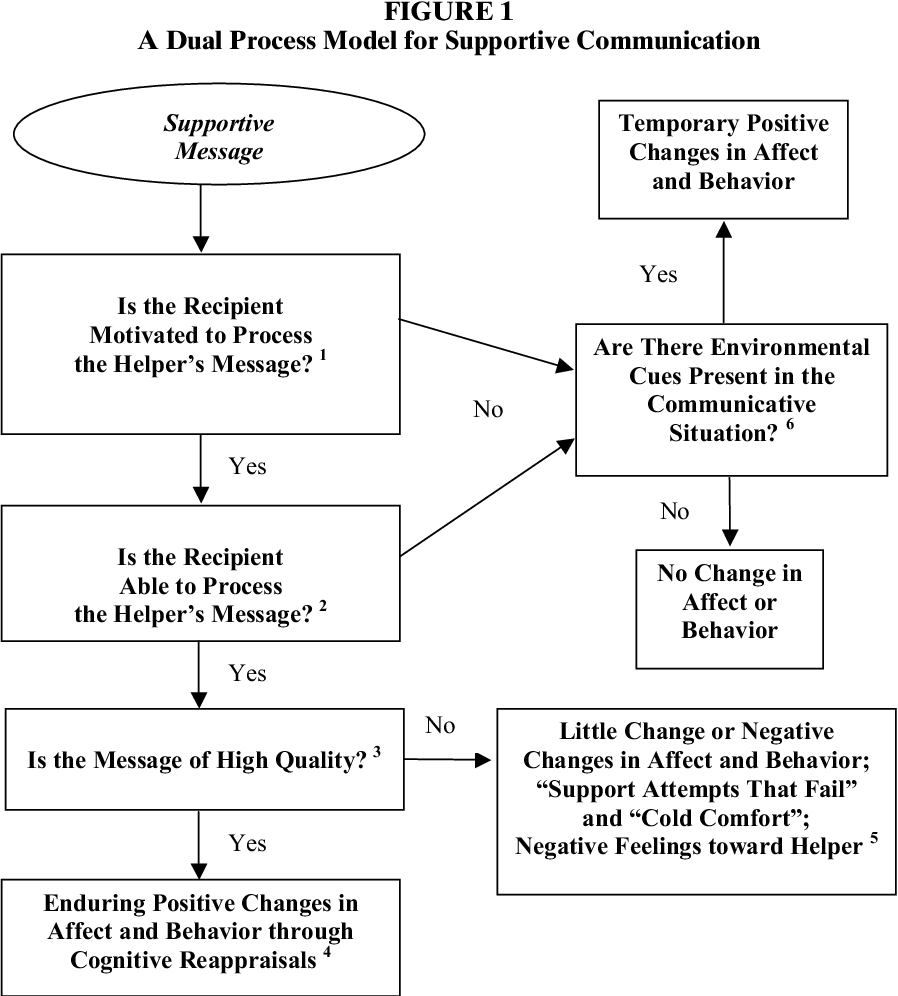
\includegraphics{images/9-Figure1-1.png}}

  \citep[pp.198]{Baxter_2008}
\end{itemize}

Modes:

\begin{itemize}
\item
  Processing modes: Elaboration (i.e., ``the extent to which an individual thinks with respect to message content'')

  \begin{itemize}
  \item
    negative affect
  \item
    motivation
  \item
    ability
  \item
    environmental cues
  \item
    Quality of supportive message: high vs.~low
  \end{itemize}
\end{itemize}

Under the framework of dual-process theory, communication is defined as ``a process in which a person (the source) seeks
to convey or make public some internal state to another (the recipient) through the use of signals and symbols (the
message) in the effort to accomplish some pragmatic end (the goal).'' \citep{burleson_2010}

Application:

\begin{itemize}
\item
  emotional support
\item
  grief management
\end{itemize}

\citep{Davis_2018} studies the microaggression of white women towards black women with two phases:

\begin{itemize}
\tightlist
\item
  Individual orientation phase (i.e., ``friends communicating verbal and nonverbal messages that solely comforted the
  support seeker'' - information seeking, support provision (e.g., the use of girls, hand clap))
\item
  Collective orientation phase (phase: Hostile differentiation, Socio-political Contextualization, Collective Uplift).
\end{itemize}

Age moderates the perceived microaggression (e.g., tolerance).

Racial microaggressions are ``brief messages (i.e., verbal, nonverbal, and visual) that denigrate people of color because
they belong to a racial group that is historically oppressed in the U.S.'' \citep{Sue_2007}

Strong Black Woman Collective Theory argues that ``strength is valuable resource for Black women because it helps them
resist external hostilities.'' \citep{Davis_2014}

\hypertarget{advice-response-theory}{%
\subsection{Advice Response Theory}\label{advice-response-theory}}

Social cognitive theory: how advice outcomes are influenced by qualities of messages, advisors, situations, and
recipients.

\textbf{Goals}:

ART predicts how your friend is likely to respond, based on your friend's perceptions of

\begin{enumerate}
\def\labelenumi{\arabic{enumi}.}
\item
  Message features (e.g., content and style): Recipients evaluate

  \begin{enumerate}
  \def\labelenumii{\arabic{enumii}.}
  \item
    message content

    \begin{itemize}
    \tightlist
    \item
      efficacy (i.e., if the action is likely to resolve the problem)
    \item
      feasibility (i.e., capacity to accomplish eh action)
    \item
      limitation
    \item
      confirmation (whether he action is consistent with the recipient's intent)
    \end{itemize}
  \item
    Style:

    \begin{itemize}
    \tightlist
    \item
      politeness
    \item
      linking
    \item
      respect
    \end{itemize}
  \end{enumerate}
\item
  Advisor's characteristics (likely to be mediated by message content)

  \begin{itemize}
  \tightlist
  \item
    Expertise (to the problem)
  \item
    trustworthiness
  \item
    likability
  \item
    similarity (to the recipient).
  \end{itemize}
\item
  Situational factors (this is controversial because of conflicting empirical evidence)

  \begin{itemize}
  \tightlist
  \item
    problem seriousness (perceived by the recipient)
  \item
    solution uncertainty (about how to resolve the problem)
  \end{itemize}
\item
  Recipient's traits or characteristic

  \begin{itemize}
  \tightlist
  \item
    thinking style
  \item
    abilities (e..g, cognitive complexity)
  \item
    demographic (e.g., culture, gender)
  \end{itemize}
\end{enumerate}

\hypertarget{interactiondiscourse-centered}{%
\chapter{Interaction/discourse Centered}\label{interactiondiscourse-centered}}

\hypertarget{evolutionary-theories}{%
\section{Evolutionary Theories}\label{evolutionary-theories}}

theoretical framework to study biology and interpersonal communication (i.e., biosocial approach)

Some traits remain relatively stable in species.

Five principles:

\begin{enumerate}
\def\labelenumi{\arabic{enumi}.}
\item
  Basic Theory of evolution: ``perpetual change in the living world where nothing is constant or repeated exactly''
\item
  Common decent
\item
  Multiplication of species
\item
  gradualism
\item
  natural selection

  \begin{enumerate}
  \def\labelenumii{\arabic{enumii}.}
  \item
    Individuals are variable. (i.e., variation among organism in the same familial lineage)
  \item
    Advantageous traits are passed on to off-spring.
  \item
    Individuals produce more offspring than the environment can support. Then, scarcity of resources kick in to
    favor individuals that have traits more advantages in acquiring resources (i.e., Adaptation), which operates at
    the genetic level (not individual).
  \item
    traits are passed on gradually which lead to new species in the population
  \end{enumerate}
\end{enumerate}

\citep{Tooby_2015} evolutionary psychology study the functions of brain, which is known as psychological adaptation that
evolve to solve problems in its environment.

Limitation:

\begin{itemize}
\tightlist
\item
  Controversial regarding sex (i.e., biological make-up of men and women are different). Biological determinism is in
  contrast to ``bi-directional nature of hormonal responses and the fact that individuals' communication can influence
  their physiological responses and vice versa.''
\item
  Controversial over culture and individual differences:
\end{itemize}

Application:

\begin{itemize}
\tightlist
\item
  \citep{Denes_2016} ``high testosterone/no orgasm individuals may be the least likely to experience the beneficial effects
  of post sex communication.''
\item
  \citep{Aloia_2014} ``positive association between conflict intensity and cortisol reactivity, and this association was
  attenuated for individuals who reported higher, rather than lower, levels of childhood exposure to familial verbal
  aggression.''
\end{itemize}

\hypertarget{affection-exchange-theory}{%
\subsection{Affection Exchange Theory}\label{affection-exchange-theory}}

(AET) \citep{Floyd_2001} contemplates that ``people give and receive affection in ways that are adaptive or evolutionarily
advantageous for their relationship.'' There is evidence that affection reduces stress.

Assumptions of AET:

\begin{itemize}
\tightlist
\item
  procreation and survival are superodinate human goals
\item
  Communication helps achieve these goals (consciously or unconsciously)
\item
  traits that are desirable (i.e., advantageous) for superordinate goals will be passed on
\item
  human communicative behaviors are only partially controlled by humans.
\end{itemize}

AET's propositions:

\begin{itemize}
\item
  ``the need and capacity for affection are inborn''

  \begin{itemize}
  \item
    we don't need to learn to feel affection(i.e., innate)
  \item
    the need for affection is fundamental
  \end{itemize}
\item
  ``affectionate feelings and affectionate expression are distinct experiences that often, but need not, covary''
\item
  ``affectionate communication is adaptive with respect to human viability and fertility''
\item
  ``humans vary in their optimal tolerances for affection and affectionate behavior''
\item
  ``affectionate behaviors that violate the range of optimal tolerance are physiologically aversive''
\end{itemize}

\citep{Floyd_1998} propose 3 forms of affection display:

\begin{itemize}
\tightlist
\item
  Verbal communication (e.g., spoken or written)
\item
  Direct nonverbal (e.g., nonlinguistic or paralinguistic behaviors)
\item
  Indirect Nonverbal (e.g., behaviors that convey affection via social or material support)
\end{itemize}

Types of affectionate communication research:

\begin{itemize}
\item
  Relationships: certain relationships are more affectionate than others because it relates to the relatedness of
  genes' survivability

  \begin{itemize}
  \item
    fathers gives more attention to children with higher probability to reproduce.
  \item
    ``humans engage in affectionate behaviors, both genuinely and deceptively, within selective romantic
    relationships in order to increase relational trust, closeness, and satisfaction.'', which in turn, increase
    survival and procreation.
  \end{itemize}
\item
  Health

  \begin{itemize}
  \item
    One can have health benefits by offering affection.
  \item
    ``highly affectionate people report higher self-esteem, general mental health, social engagement, and life
    satisfaction,a s well as lower susceptibility to depression and stress, than less-affectionate
    people''\citep{Floyd_2002}
  \end{itemize}
\end{itemize}

Application:

\citep{Floyd_2009}

\begin{itemize}
\tightlist
\item
  kissing improves perceived stress, relationship satisfaction, and total serum cholesterol
\end{itemize}

\citep{Horan_2013}

\begin{itemize}
\item
  motivation for deceptive affection:

  \begin{itemize}
  \item
    face-saving
  \item
    conflict management/ avoidance
  \item
    emotion management
  \end{itemize}
\item
  feelings of affection is different from communicating affection

  \begin{itemize}
  \item
    feeling affection: the feeling of warmth and fondness toward an individual
  \item
    communicating affection: feelings of fondness, support, and love
  \end{itemize}
\end{itemize}

\citep{Davis_2019}

\begin{itemize}
\item
  Controlling images (.e.g, angry black woman or mammy). Black women are thought to be self-sufficient, perseverant,
  authentic.
\item
  Strong Black woman collective theory: ``Black women enact communication behaviors that affirm strength in each other
  \ldots{} to delineate a safe space to concurrently promote solidarity within the collective and confront oppressive
  force.''

  \begin{itemize}
  \item
    Black women use ``distinct communication practices (i.e., code-switching, assertive and verbal messages, and
    culturally-nuanced speech codes)''
  \item
    the assemblage of Black women
  \item
    members reinforce each others virtues of strength
  \item
    enable members to confront oppressive structure, but also impede vulnerability and emotionality within
  \end{itemize}
\item
  Strength regulation like emotion regulation
\item
  ``strength regulation contributed to more derogative comments about aggressors during supportive discussions, and
  support seekers were less satisfied in their relationships with white women after the derogative conversations''
\end{itemize}

\citep{Gilchrist_Petty_2019}

\begin{itemize}
\tightlist
\item
  engaged-to-be-married has the highest negative attitudes regarding cross-sex best friendships.
\item
  attitudes toward cross-sex best friendships mediate the relationship between (how jealousy experienced and
  expressed) and (reactive jealousy experience and destructive jealousy expression)
\end{itemize}

\hypertarget{tend-and-befriend-theory}{%
\subsection{Tend and Befriend theory}\label{tend-and-befriend-theory}}

Under the fight or flight framework, people tend to affiliate with others under stress \citep{Taylor_2012}. Women have
different level of fight or flight tendencies, which is due to hormones and evolutionary tendencies.

\hypertarget{attachment-theory}{%
\subsection{Attachment theory}\label{attachment-theory}}

\citep{Bowlby_1982} As child, we form attachments to our parents, which affect how we perceive and approach relationship in
the future. Oxytocin is a hormone that facilitates social bonds \citep{Campbell_2010}

\hypertarget{intergroup-theorizing}{%
\section{Intergroup Theorizing}\label{intergroup-theorizing}}

\hypertarget{communication-accommodation-theory}{%
\subsection{Communication Accommodation Theory}\label{communication-accommodation-theory}}

Varying communicative styles are reflections of personalities, roles, temperaments, and social identities.

Communication Accommodation theory (CAT) explains why we communicate differently with different people (i.e., our
communication choices change based on the relational, identity we engage in).

Accommodation is ``a process concerned with how we can reduce (and, in some cases, even magnify) communicative
differences between people in interaction'' \citep[pp.~237]{Baxter_2008}. It ``enhances interpersonal similarities, and reduces
uncertainties about the other'' \citep[pp.~237]{Baxter_2008}. Speakers will be seen as more competent and credible
\citep{Aune_1993}. Accommodation manifests via convergence in language (i.e., dialect), nonverbal cues (e.g., speech rate,
posture) \citep{Li_2001}. Those with more social power are often accommodated. \emph{(however, I think less social power should be
accommodated, for example, patients and doctors, benefactors and beneficiaries)}

Nonaccommodacaiton can signal lack of respect or liking to the other person (could be intentional or unintentional), or
authenticity. Divergence signal membership in groups, culture, and communities (their social identity).

Symmetricality and accommodation lead to strengthened interpersonal relations, and vice versa.

Principles of accommodation:

\begin{enumerate}
\def\labelenumi{\arabic{enumi}.}
\item
  Speakers will, up to an optimal level, increasingly accommodate the communicative patterns believed characteristic
  of their interactants the more they wish to

  \begin{enumerate}
  \def\labelenumii{\arabic{enumii}.}
  \item
    Signal positive face and empathy
  \item
    Elicit the other's approval, respect, understanding, trust, compliance, and cooperation
  \item
    Develop a closer relationship
  \item
    Defuse a potentially volatile situation
  \item
    Signal common social identities
  \end{enumerate}
\item
  When attributed (typically) with positive intent, patterns of perceived accommodation increasingly and cumulatively
  enhance recipients'

  \begin{enumerate}
  \def\labelenumii{\arabic{enumii}.}
  \item
    Self-esteem;
  \item
    Task, interactional, and job satisfaction;
  \item
    Favorable images of the speaker's group, fostering the potential for partnerships to achieve common goals;
  \item
    Mutual understanding, felt supportiveness, and life satisfaction;
  \item
    Attributions of speaker politeness, empathy, competence, benevolence, and trust.
  \end{enumerate}
\item
  Speakers will (other interactional motives notwithstanding) increasingly nonaccommodate (e.g., diverge from) the
  communicative patterns believed characteristic of their interactants, the more they wish to signal (or promote)

  \begin{enumerate}
  \def\labelenumii{\arabic{enumii}.}
  \tightlist
  \item
    Relational dissatisfaction or disaffection with and disrespect for the others' traits, demeanor, actions, or
    social identities.
  \end{enumerate}
\item
  When attributed with (usually) harmful intent, patterns of perceived nonaccommodation (e.g., divergence) will be

  \begin{enumerate}
  \def\labelenumii{\arabic{enumii}.}
  \item
    Evaluated unfavorably as unfriendly, impolite, or communicatively incompetent;
  \item
    Reacted to negatively by recipients (e.g., recipients will perceive speaker to be lacking in empathy and trust)
  \end{enumerate}
\end{enumerate}

CAT absorbs both interpersonal and intergroup process, even though they are considered orthogonal.

Application:

\citep{Chen_2016}

\begin{itemize}
\item
  The characteristics of their communication partner (mediated by specific communication behaviors imagined by the
  participant for two of the three trait dimensions such as overaccommodation for perceptions of competence, humorous
  communication for perceptions of sociability) influences participants' stereotypes of older adult

  \begin{itemize}
  \tightlist
  \item
    overaccommendation can be seemed patronizing, which reinforces stereotypes
  \end{itemize}
\item
  Imagined interaction involves individuals' spontaneous thoughts regarding interpersonal communication with a real
  person, which typically occurs before an actual interaction with the person \citep{Honeycutt_2014}.
\item
  based on stereotype content model (SCM), groups are stereotyped based on two dimensions: warmth and competence
  \citep{Fiske_2007}. Later warmth was further segmented into sociability and morality (i.e., trustworthiness)
\end{itemize}

\hypertarget{communication-theory-of-identity}{%
\subsection{Communication Theory of Identity}\label{communication-theory-of-identity}}

Stem from psychology and sociology in the 50s and 60s. ``Similar to the psychological tradition, the self was still most
often discussed in unitary terms with social roles reserved for the various different manifestations'' \citep[pp.
254]{Baxter_2008}.

There isn't one core genuine self, but multiple selves (i.e., multiple identities). Self emerges out of one's social
interactions and the perceptions of others \citep{stryker1979}.

Identity/Communication (identity is not separable from communication) leads to communication satisfaction.

CTI conceptualizes layers of identity as both changing and stable, and both subjective and ascribed. 4 layers are
interdependent:

\begin{itemize}
\tightlist
\item
  Personal: individual, sense of self-being
\item
  relational: identity defined in relationship, and ascribed
\item
  Enacted: performance of identity, through verbal and nonverbal messages
\item
  Communal: how society defines identity and identities (i.e., group membership)
\end{itemize}

The gap between personal and enacted identities is called identity gaps \citep{Jung_2004}, leads to negative psychological
outcomes (e.g., depression). But it could also help individual try to close the gap (cognitive dissonant).

We want others to value the same attributes that we ourselves value \citep[pp.~261]{Baxter_2008}

\hypertarget{application}{%
\subsubsection{Application}\label{application}}

\citep{WILLER_2010}

\begin{itemize}
\item
  Socially aggressive face threats (SAFTs) are ``messages that threaten one's identity or positive face''
\item
  social aggression can damage self-esteem, social standing.
\item
  Face is the self or image that people present and expect others to main or support during interaction
  \citep{Cupach_1994}, which includes two desires:

  \begin{itemize}
  \item
    positive face needs: desire for approval, appreciation, and liking
  \item
    negative face needs: desires for freedom from action ad imposition
  \end{itemize}
\item
  and two threats

  \begin{itemize}
  \tightlist
  \item
    positive face threats: similar to socially aggressive messages. Hence, the authors use the terms SAFTs.
  \end{itemize}
\item
  Negative affect negatively associated feelings of forgiveness (measured by feelings of revenge and avoidance,
  avoidance)
\end{itemize}

\citep{Nuru_2014}

\begin{itemize}
\item
  transgender is when ``self-identify with a gender that `'contradicts'' socially acceptable gender roles and
  expectations as dictated by external genitalia and assigned birth sex.''

  \begin{itemize}
  \tightlist
  \item
    ``any divergence from conventional social norms that tie gender identity to role expectancy and biological sex''
    \citep{Bornstein_2013}
  \end{itemize}
\item
  Gender identity may overlap sexuality, they are two distinct processes of negotiation.
\item
  Genital sex can differ from social and psychological gender.
\item
  Gaps between personal, enacted, and relational layers are prevalent.
\item
  Strategies to mitigate tension:

  \begin{itemize}
  \item
    Closeted enactment
  \item
    disengagement
  \item
    passing: intentional disguise to preserve relationship
  \item
    label changing
  \end{itemize}
\end{itemize}

\citep{Harris_2018}

\begin{itemize}
\item
  In the context of bullying, studies have traditionally been White-oriented. Hence, there is a need for diverse
  sampling.
\item
  Due to political climate in 2016, students are reported to be more anxious and new wave of political bullying was on
  the rise.
\item
  race is a social construct that relates to power, privilege, and systemic oppression. racist draw societal power
  from being members of the majority group. Racism is different from racial prejudice and racial discrimination (i.e.,
  everybody can be racially prejudice, but only macro culture members can be racists).
\item
  Bullying can happen between group (macro vs.~micro cultures), and within group (in-group bullying, i.e., Mexican
  American and Mexican immigrants).
\item
  Marginalized status triggers victim status

  \begin{itemize}
  \tightlist
  \item
    family socioeconomic status (SES) and test scores are correlated
  \end{itemize}
\item
  Intersectioanality and Race in Bullying
\end{itemize}

\hypertarget{critical-approaches-to-ipc-research}{%
\section{Critical Approaches to IPC Research}\label{critical-approaches-to-ipc-research}}

List of interpersonal communication theories under critical approaches:

\begin{itemize}
\tightlist
\item
  Relational dialectics Theory
\item
  Narrative performance Theory
\item
  Family of Feminist theories
\end{itemize}

Difference between postmodern critical approach and modern tradition is how power is conceptualized, but both agree that
power has impact on communicative life with the goals of emancipation and empowerment.\\
Critical modern hope to free people from socially oppressed system, but postmodern critical scholars view the world as
constant struggle for dominant discourses.

Power definition:

\begin{itemize}
\tightlist
\item
  Post-positivistic tradition: ``as an individual level variable based on the various kinds of resources the individual
  posses'' (Berger, 1994).
\item
  modern critical: ``as a systemic construct that exists external to the individuals who operate within those systems.''
  \citep[pp.~273]{Baxter_2008}
\end{itemize}

Critical Modern Tradition:

\begin{itemize}
\item
  False consciousness: lack of awareness of constraints imposed by system (Pine, 1993).
\item
  goal: dismantle false consciousness to free people
\item
  Communication is a reflection of systematic constraint
\item
  Application:

  \begin{itemize}
  \item
    Gender as a social system, gender is a range of ideals (masculine and feminism).
  \item
    Relational Labor as a social system
  \end{itemize}
\end{itemize}

Postmodern Tradition

\begin{itemize}
\item
  Resist thinking of power as top-down, and advocate for power is bottom-up-and-out dynamics and power is constantly
  met with resistant, which means it is unstable and fluid.
\item
  Comminciaiton is the social world (not a reflection of it).
\item
  Application:

  \begin{itemize}
  \item
    Uncertainty as positive precondition for change
  \item
    Self-making instead of Self-disclosure: individuals are not intact.
  \end{itemize}
\end{itemize}

To evaluate critical approaches to interpersonal communication, we need to consider:

\begin{itemize}
\tightlist
\item
  ethics: (1) how your position impacts what is identifiable, and that which is beneficial
\item
  change: can your change emancipate the marginalized and oppressed?
\end{itemize}

\hypertarget{critical-feminist-theories}{%
\section{Critical Feminist Theories}\label{critical-feminist-theories}}

\begin{itemize}
\item
  Feminist Theories

  \begin{itemize}
  \item
    ``Feminism'' is ``defined as the belief that men and women are equal and should have equal rights and
    opportunities in all spheres of life---personal, social, work, and public''. \citep[pp.~290]{Baxter_2008}

    \begin{itemize}
    \item
      Gender (different from sex): social meaning attached to biological distinct, which is embedded in
      communication
    \item
      Patriarchy: " a system that reflects primarily the interests, values, perspectives, and experiences of men,
      as a group." \citep[pp.~290]{Baxter_2008}
    \end{itemize}
  \end{itemize}
\item
  Critical Theories:

  \begin{itemize}
  \tightlist
  \item
    "identify prevailing structures and practices that create or uphold disadvantage, inequity, or oppression, and
    to point the way toward alternatives that remote more egalitarian relationships, groups, and societies.
    \citep[pp.~292]{Baxter_2008}
  \end{itemize}
\item
  The production of the two theories:

  \begin{itemize}
  \tightlist
  \item
    The recursive relationship between how cultural structures and practices differently and inequitably shape
    women's and men's lives and communication practice and vice versa.
  \end{itemize}
\item
  Assumptions:

  \begin{itemize}
  \tightlist
  \item
    ``members of groups defined by sex, race, and other factors occupy distinct positions in a society - those are
    their social location.''
  \end{itemize}
\item
  Methodological Implication: examination of power that is both formal and informative ones.
\item
  Power:

  \begin{itemize}
  \tightlist
  \item
    in relation to unequal status, privilege.
  \end{itemize}
\item
  Communication: with less communication on a subject, we'd have less knowledge of it, or even notice it.

  \begin{itemize}
  \tightlist
  \item
    Hence, we should name and increase social awareness of women's experiences.
  \end{itemize}
\item
  Examples

  \begin{itemize}
  \item
    Sexual harassment
  \item
    Date rape
  \item
    Marital rape
  \item
    Second Shift
  \item
    Conversational maintenance work
  \end{itemize}
\item
  Evaluation:

  \begin{itemize}
  \item
    Parsimonious: few concepts (gender, power, dominance).
  \item
    Limited explanability since it focuses on sex and gender, and limited utility: small subset of people.
  \end{itemize}
\end{itemize}

Application:

\citep{Sanford_2019}

\begin{itemize}
\tightlist
\item
  Based on Co-Cultural Theory, the authors found that even when they constitute a large part of an institution's
  population, Hispanic students still feel the need to behave under White norms (assimilationist strategies).
\end{itemize}

\citep{Ross_2016}

\begin{itemize}
\tightlist
\item
  Modification s to office logistic and and practitioners' behavior can increase a healthy communication environment
  among trans-patient-practitioner
\end{itemize}

\citep{Nuru_2018}

\begin{itemize}
\item
  memorable messages about race:

  \begin{itemize}
  \item
    denial of racism
  \item
    preparation for bias
  \item
    promotion of mistrust
  \end{itemize}
\item
  these memorable message help make sense of racial hierarchies in Cost Rica and racial socialization in the global
  contexts.
\end{itemize}

\citep{Suter_2017}

Critical Interpersonal and Family Communication framework should consider:

\begin{itemize}
\tightlist
\item
  power
\item
  bi-directionality between private and public realms
\item
  critique/resistance/transformation of the status quo in the service of social-justice ends
\item
  author reflexivity
\end{itemize}

``(a) What is my impetus for speaking and writing? (b) Where am I speaking from? (c) To whom am I accountable in this
process? (d) What are the potential material and discursive effects resulting from my speaking and writing'' (Yep, 2010,
p.~173)

\hypertarget{relationship-centered}{%
\chapter{Relationship Centered}\label{relationship-centered}}

\hypertarget{affection-exchange-theory-1}{%
\section{Affection Exchange Theory}\label{affection-exchange-theory-1}}

\hypertarget{transnational-scholarship}{%
\section{Transnational Scholarship}\label{transnational-scholarship}}

\hypertarget{resilience-communication-theories}{%
\section{Resilience Communication Theories}\label{resilience-communication-theories}}

\citep{Buzzanell_2010}

\begin{itemize}
\item
  Human resilience is ``the ability to''bounce back" or reintegrate after difficult life experiences"
\item
  Resilience is not possessed by individual but by discourse, interaction, and processes:

  \begin{itemize}
  \item
    crafting normalcy
  \item
    affirming identity anchors:

    \begin{itemize}
    \tightlist
    \item
      identity anchor is ``a relatively enduring cluster of identity discourses upon which individuals and their familial, collegial, and/or community members rely when explaining who they are for themselves and in relation to each other.''
    \end{itemize}
  \item
    maintaining and using communication networks

    \begin{itemize}
    \tightlist
    \item
      Social capital is important in time of need
    \end{itemize}
  \item
    putting alternative logics to work
  \item
    downplaying negative feelings while foregrounding positive emotions
  \end{itemize}
\item
  \citep{Richardson_2002} defines resilience as ``the process of reintegrating from disruptions in life''

  \begin{itemize}
  \tightlist
  \item
    requires ``trigger event''
  \end{itemize}
\end{itemize}

\citep{AFIFI_2016}

\begin{itemize}
\item
  Theory of resilience and relational load (TRRL) in the context of social

  \begin{itemize}
  \item
    based on theory of

    \begin{itemize}
    \item
      emotional capital
    \item
      adaptive calibration model, allostatic load, investment model, family systems theory, affectionate exchange theory, broaden and build theory
    \end{itemize}
  \item
    Assumptions

    \begin{itemize}
    \item
      people want to feel validated and secure, based on sociometer hypothesis, intergroup theories, social identity theory, evolutionary theories (e.g., exchange theory).
    \item
      stress is natural and necessary (either good or bad).

      \begin{itemize}
      \item
        good stress = positive perception of stressors
      \item
        bad stress = distress = negative perception of stressors
      \end{itemize}
    \item
      body and mind work together to cope with stress
    \item
      body has a natural diurnal rhythm
    \item
      relationship have homeostasis that is ``continually being calibrated in response to stress and the communication of stress.''
    \end{itemize}
  \item
    Propositions:

    \begin{itemize}
    \item
      ``Validating communicative maintenance behaviors and actions over time build positive emotional reserves. Emotional reserves reflect the accumulation of investments (i.e., maintenance) and discrepancies in investments''
    \item
      Communal orientation \& discrepancies influence communication maintenance behaviors/discrepancies, and vice versa
    \item
      Communal orientation, emotional reserves, discrepancies in the communal orientation influence how one perceives stressors, which later influence their investment in the relationship
    \item
      communal orientation and emotional reserves, discrepancies int eh communal orientation influence threat and security-based appraisals and communication pattern

      \begin{itemize}
      \item
        Similar constructs to communal orientation are cognitive interdependence, couple identity, communal coping
      \item
        self-control could be depleted
      \end{itemize}
    \item
      continued depletion of resources and increased stress increase relational load
    \item
      short-term depletion and relation load have short-term and long-term health consequences respectively.
    \item
      ``Security-based appraisals and communication patterns facilitate resilience, the potential to thrive, and short-term and long-term health''
    \item
      Communicative maintenance strategies can be learned
    \end{itemize}
  \end{itemize}
\item
  Resilience is ``the ability to adapt positively when confronted with adversity or stress'' \citep{2003_3713}
\item
  positive \emph{relationship maintenance} can serve as resilience in close relationships, via

  \begin{itemize}
  \item
    nonverbal behaviors
  \item
    perceptions
  \end{itemize}
\end{itemize}

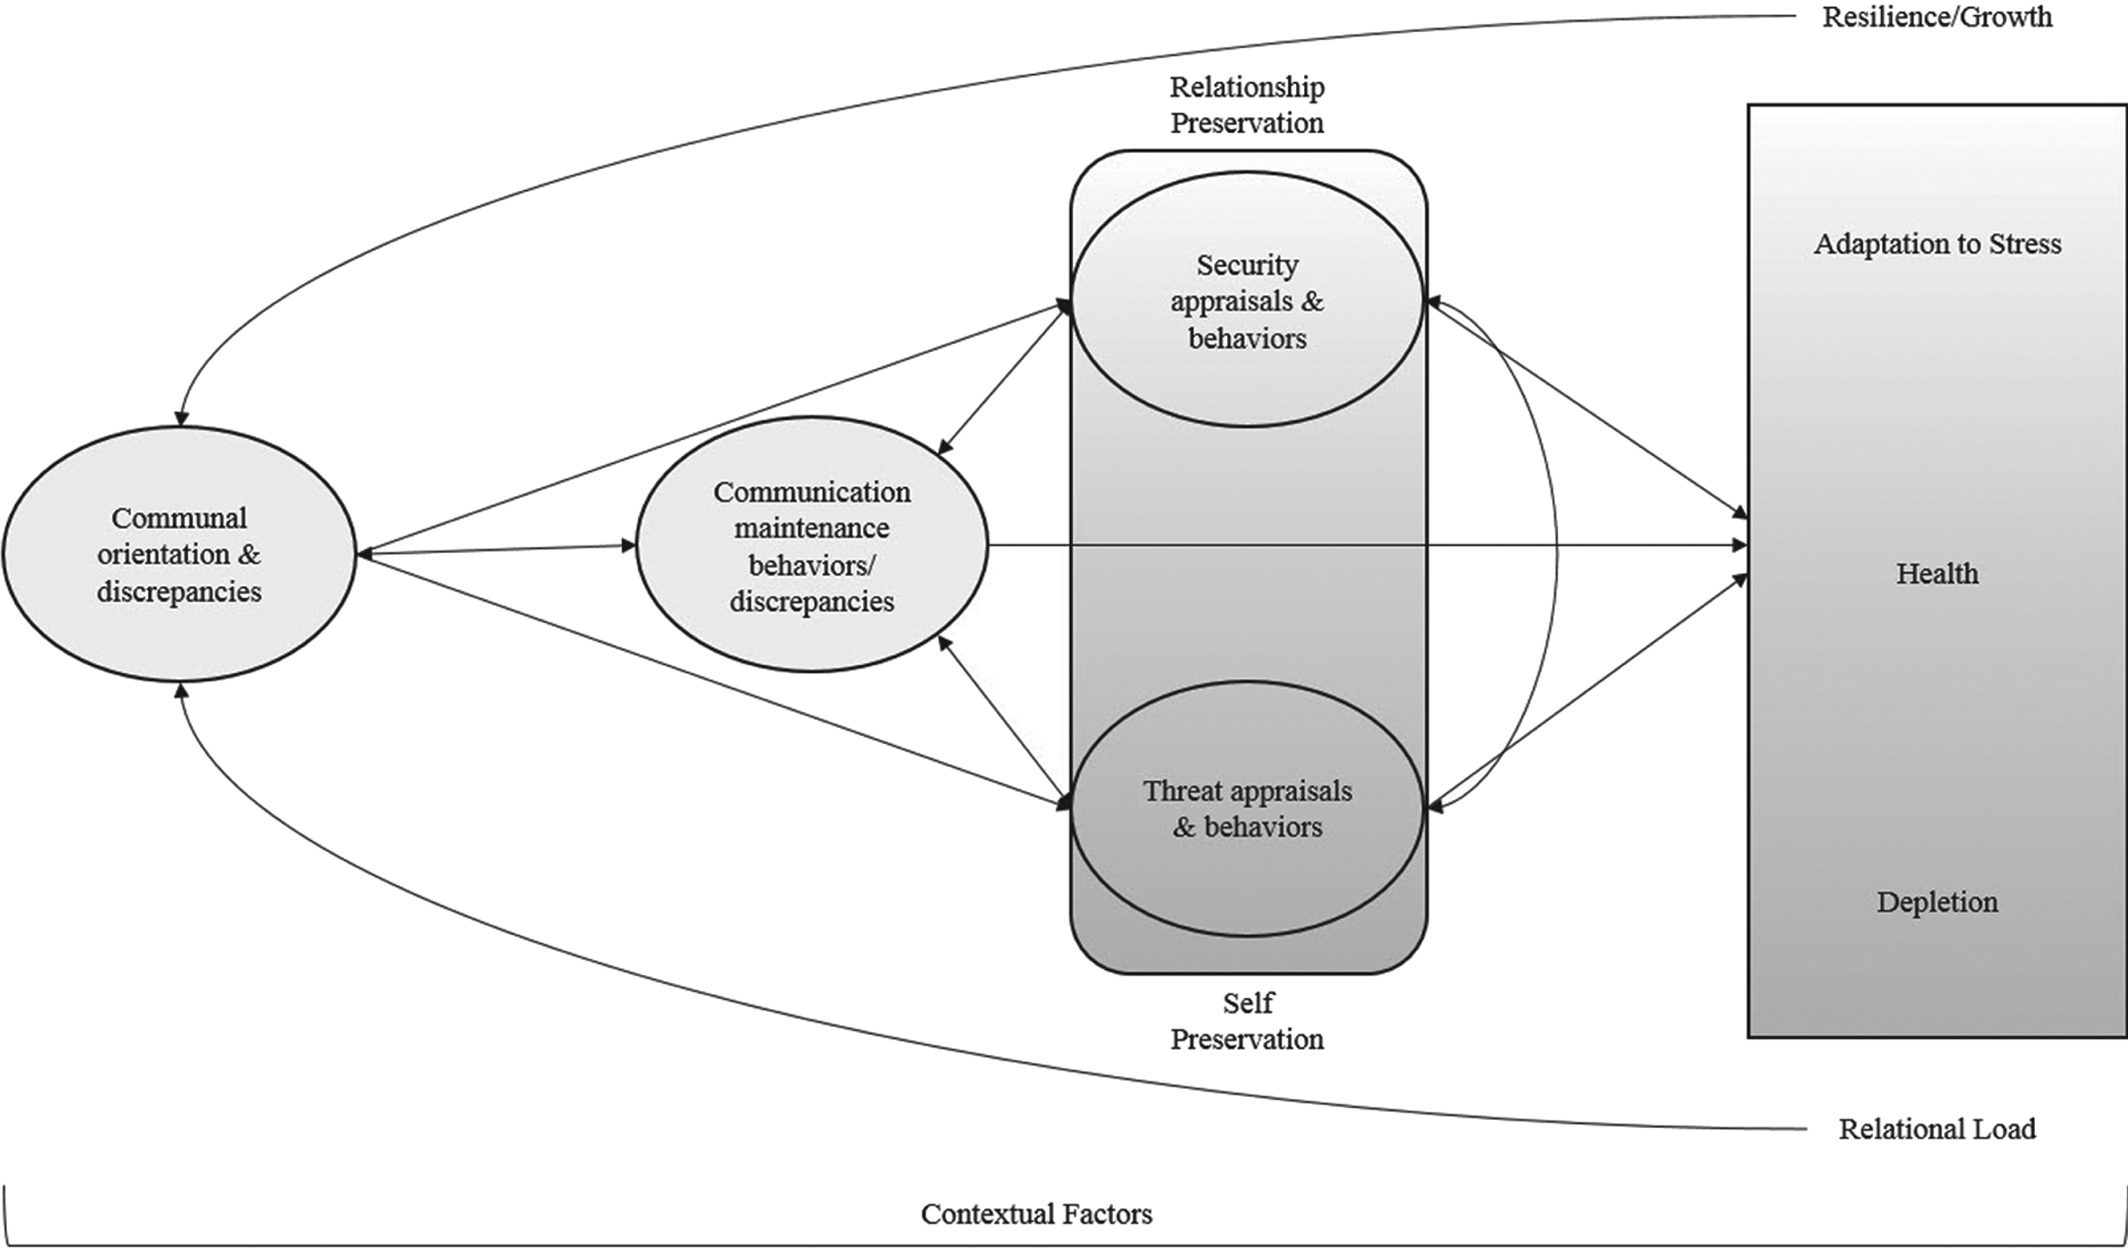
\includegraphics{C:/Users/tn9k4/GitHub/comm_theory/images/theory of resilience and relational load.jpg}

Picture from \textbf{Personal Relationships, Volume: 23, Issue: 4, Pages: 663-683, First published: 26 October 2016, DOI: (10.1111/pere.12159)}

\citep{Buzzanell_2018}

Resilience include:

\begin{itemize}
\item
  Individual/relational resilience: social relationship can increase adaptive ability to adversity. To increase one's resilience

  \begin{itemize}
  \item
    giving and receiving affection
  \item
    exchanging person-centered messages
  \item
    being present
  \end{itemize}
\item
  family resilience

  \begin{itemize}
  \tightlist
  \item
    parent-child (dyadic) can foster resilience
  \end{itemize}
\item
  organizational resilience

  \begin{itemize}
  \tightlist
  \item
    5 tensional processes
  \end{itemize}
\item
  community resilience

  \begin{itemize}
  \tightlist
  \item
    bouncing forward = interactional process that helps individuals to adapt successfully to changing circumstances
  \end{itemize}
\item
  national resilience

  \begin{itemize}
  \tightlist
  \item
    resilience is defined by Hamilton Bean as a ``central trope'', ``shared social phenomenon'' that solidify ``shared feelings of resoluteness.''
  \end{itemize}
\end{itemize}

\citep{Kam_2018}

\begin{itemize}
\item
  How undocumented youth cope with stress at the family level
\item
  Resilience is ``the process by which individuals exposed to adversity exhibit
  positive adaptation in spite of this adversity.'' It is a general pattern or process than a trait or quality.
\item
  To cope with stress, youths use strategies:

  \begin{itemize}
  \item
    psychological suppression
  \item
    distraction/diversion
  \item
    reframing
  \item
    normalizing
  \end{itemize}
\item
  The individual as an asset
\item
  The family as a resource
\item
  Stress come from

  \begin{itemize}
  \item
    unable to go places, unable to attend college, employment, help family financially, affordable health care
  \item
    fear of detainment/deportation
  \end{itemize}
\end{itemize}

\citep{First_2020}

\begin{itemize}
\tightlist
\item
  Covid-19 exposure directly influence stress, and indirectly influence stress and depress through media use and interpersonal communication.
\end{itemize}

\hypertarget{communication-privacy-management-theory}{%
\section{Communication Privacy Management Theory}\label{communication-privacy-management-theory}}

\hypertarget{relational-turbulence-theory}{%
\section{Relational Turbulence Theory}\label{relational-turbulence-theory}}

\hypertarget{part-organizational-communication}{%
\part{ORGANIZATIONAL COMMUNICATION}\label{part-organizational-communication}}

\hypertarget{perspectives-on-organizational-communication}{%
\chapter{Perspectives on Organizational Communication}\label{perspectives-on-organizational-communication}}

\citep{Mumby_1996}
Organizational communication as a discipline can be looked under the framework of 4 problematics.

The problematic of:

\begin{enumerate}
\def\labelenumi{\arabic{enumi}.}
\tightlist
\item
  voice: characterized by multiple voices, not only managerial.\\
  + organizational communication cultivates tensions between university and firms, rather than resolving it.\\
  + how voices can gain insight into marginalized groups.\\
\item
  rationality\\
  + pluralist understandings
  + technical rationality: ``knowledge that privileges a concern with prediction, control and teleological forms of behavior''.\\
  + Practical rationality: ``knowledge grounded in the human interest in interpreting and experiencing the word as meaningful and intersubjectively constructed''\\
\item
  organization\\
  + The question of organization is fundamental in organizational communication.\\
  + the complex structure of organizing, culture and larger social processes.\\
\item
  organization-society relationship\\
  + organizational boundaries (separation between organization and society) cannot be clearly defined due to its fluid nature.\\
  + can study the dynamics nature of globalization.\\
  + communication is not just information exchange, but it is the core of organizing where organization structure is dynamically created.
\end{enumerate}

\citep{Broadfoot_2007}~\\
We might have been myopic when only interpret and look at organizational communication from the perspective of Euro-American intellectual tradition. hence, we need to have alternative, rationalities, and perspectives.

Due to \citep{Mumby_1996}, there are four major problematics in organizational communication:

\begin{itemize}
\tightlist
\item
  Voice: who gets to speak for whom\\
\item
  Rationality: 2 forms of rationalities: technical/instrumental and practical and the consequences.\\
\item
  Organization: members create meaning through communication.\\
\item
  Organization-society relationship: it's hard to distinguish between the two, hence we should study in conjunction.
\end{itemize}

there is a new shift to the non-American voices: A Postcolonial awakening.

Postcolonial self-reflexivity: a resistance from Eurocentric perspective.

\citep{Shome_1996} defines Discursive confinement as ``a state where difference and individuality are eased or neutralized and scholars become confined to a narrow and marginalized discursive space constructed by dominant mainstream structures and ideologies''. Hence, we should break through the discipline and embed individuality through emotionality.

We can see the shift in areas such as gender, race, and globalization.

A postcolonial exploration: different perspective can contribute richly to the understanding organizational communication.

\citep{Cheney_2007}

Identity: from business. flow of information between stakeholders.

Breaking boundaries: expand to other issues such as informal network, social movements, etc.

Opportunities from social problems: shift from basic research to focus on society and planet.

Ethos and Confidence: The discipline of organizational communication as well as communication are constantly in need to prove for its legitimacy.

Audiences: various outlets, but mostly focus on research publication due to the need for tenure.

To get beyond the pressure for tenure, the author suggests:

\begin{itemize}
\tightlist
\item
  choose an issue that you care.\\
\item
  listen/read well from various perspectives\\
\item
  choose appropriate outlets.\\
\item
  set everyday goal.\\
\item
  practice what you preach\\
\item
  lead by example\\
\item
  do not give up\\
\item
  pause and reflect.
\end{itemize}

\citep{DUrso_2014}

History (genealogy) of organizational communication with the method of network analysis.

Author posted several research questions that could use the network analysis method to probe into such as collaboration and coauthorship, and overall development of organizational communication.

\citep{Leonardi_2016}

the strategy of subordination taken by organizational communication researchers are those that look at a phenomena from the perspective of organizational communication, which leads to small contribution to the literature.

To know if a one owns a phenomenon is when people know to turn to you when they wan to understand such phenomenon .

\hypertarget{strategy-of-discovery}{%
\subsection{Strategy of Discovery}\label{strategy-of-discovery}}

2 steps:

\begin{enumerate}
\def\labelenumi{\arabic{enumi}.}
\tightlist
\item
  Phenomenon is communication\\
\item
  What communication does and why
\end{enumerate}

\hypertarget{strategy-of-reconceptualizatinon}{%
\subsection{Strategy of Reconceptualizatinon}\label{strategy-of-reconceptualizatinon}}

2 steps:

\begin{enumerate}
\def\labelenumi{\arabic{enumi}.}
\tightlist
\item
  Contradictory evidence or poor explanation\\
\item
  Communications leads to better fit (e.g., accuracy or novelty)
\end{enumerate}

\hypertarget{organizational-culture}{%
\chapter{Organizational Culture}\label{organizational-culture}}

\citep{Martin_1983}

Culture:

\begin{itemize}
\tightlist
\item
  based on history, members can behave and expected to behave\\
\item
  help construct common value for employees.\\
\item
  control mechanisms which dictate patterns of behavior
\end{itemize}

culture can hardly be under control, not monolithic phenomenon

3 levels of culture:

\begin{itemize}
\tightlist
\item
  basic assumptions\\
\item
  values/ideology\\
\item
  artifacts (e.g., stories, rituals, dress): express values\\
\item
  management practices (e.g., training program).
\end{itemize}

Types of subcultures:

\begin{itemize}
\tightlist
\item
  enhancing: same position\\
\item
  orthogonal: unrelated position\\
\item
  counterculture: opposite position: ``most likely to arise in a strongly centralized institution that has permitted significant decentralization of authority to occur'' (e.g., GM's culture: team players, loyalty, ``refrigerator story''), balancing act must be taken to manage counter culture and dominant culture
\end{itemize}

\citep{Dixon_2009}
multiple meanings of organizational culture

Consulting method: in-depth and focus group interviews with student staff, artifact analysis, and observation of organization staff meetings and retreats

Common terms did not mean the same thing. 2 different fields: organizational communication, and higher education.

\begin{itemize}
\tightlist
\item
  Organization culture: ``German approach, based in phenomenological/Interpretive epistemology''. culture is the product of symbolic interaction. Scholars tries to understand the role of human interaction. organizational culture is not easily manipulated by managers. " organization is a culture". purposes:\\
  + increasing productivity\\
  + understanding organizational processes\\
  + critiquing oppressive organizational practices.
\item
  organizational culture: American approach to study organizational variable that affect organizational effectiveness. ``organization has a culture''. can be quantified, and manipulated.\\
  + Institution can be measured: dynamism vs.~stability and internal vs.~external focus.
\end{itemize}

two subculture: First-born (tradition, consensus) and Youngest (debate, and new ideas)

The problem stems from different discipline understanding of ``culture'', there was a rejection of the definition by organizational communication scholars.

" Rather than positing that there is one ``right'' concept, we would encourage other consultants to proactively discuss with clients, what key terms mean to them in the particularity of their context, as a means of creating a ``shared discursive'' reality."

\citep{Leonardi_2008}
mergers between two technology companies

cultural studies of postmerger integration

A core technology is ``the primary technology produced, serviced, or sold by an organization''.

technological grounding suggests that ``an organization's core technologies are, along with the work and communication practices enacted daily by members, a constitutive feature of its culture''

two dominant perspectives for understanding culture that exist in organizational literature:

\begin{itemize}
\tightlist
\item
  as a variable that can be changed.\\
  + technology is a variable . The two variables are distinct and can be either internal or external based on researchers' perspective.\\
\item
  culture is organization.\\
  + in postmerger, organizations face cultural convergence.
  + technology is not a variable but a practice.
  + ``When technologies are sufficiently important to an organization to become key elements in the constitution of a culture, we refer to that organization as technologically grounded.'' (a continuum not dichotomy).\\
  + ``technological incompatibility implies the incompatibility of organizational cultures and practices''
\end{itemize}

Method: a single case design, embedded design:

levels of analysis\\
(1) public discourse from company officials about the merger,
(2) organizational practices and policies before and after the merger
(3) worker responses during postmerger integration

US West built its culture on the West culture use analog data\\
Qwest built its culture on speed use digital data (all internet protocol - IP)

Qwest consumed US West's culture (e.g., bureaucracy) due to its technological superiority and cultural superiority in postmerger integration

Qwest shut down US West's Research Labs.

\hypertarget{section}{%
\section{4}\label{section}}

Chapter 4: Communicating Organizational Culture: A Problem-Solving Model.

Communication: is about creating message, production and reproduction of meaning.

Organizations are communication.

Gestalt Theory (figure and ground): sometimes the important part is thought of as the background

Organizational culture is an active process that shape organizations.

organizational culture is defined ``as the shared communicative process through which meanings are constantly employed, negotiated, and contested to create a stable communication environment within which organizational life becomes patterned and persistent over time.''

organizational cultures does not mean shared meaning but \textbf{shared process of meaning making}.

Forms of communication:

\begin{itemize}
\tightlist
\item
  info sharing\\
\item
  message production\\
\item
  meaning making
\end{itemize}

organizational values as ``those things, standards, and ideals through which we evaluate our organizational wellbeing''.

Types of values:

\begin{itemize}
\tightlist
\item
  Personal values\\
\item
  Moral values\\
\item
  Aesthetic values\\
\item
  Status values: power allocation.
\end{itemize}

Organizational meanings

\begin{itemize}
\tightlist
\item
  Cognitive meanings\\
\item
  Emotional meanings: people might mistakenly consider irrationality as emotionality.\\
\item
  Social meanings sensemaking theory\\
\item
  Identity meanings cultural contract theory of identity. 3 types of cultural contracts:\\
  + ready-to-sign contracts: assimilation (physical, behavioral,a nd mental assumption of dominant culture).\\
  + Quasi-completed contracts: allows adaption\\
  + Cocreated contracts: mutual valuation.\\
\item
  Power meanings\\
  + can derived from formal hierarchy\\
  + or from relationships (as opposed to isolation).
\end{itemize}

\hypertarget{sensemaking}{%
\chapter{Sensemaking}\label{sensemaking}}

Sensemaking is ``how organizational members come to understand and move forward when faced with unexpected or
unanticipated information'' (Dougherty, 2020)

\begin{itemize}
\tightlist
\item
  It can help stabilize the organization in time of crisis.
\end{itemize}

The difference between sensemaking theory and \protect\hyperlink{uncertainty-management-theory}{Uncertainty Management Theory}: they are close ties.

\begin{longtable}[]{@{}ll@{}}
\toprule
\begin{minipage}[b]{(\columnwidth - 1\tabcolsep) * \real{0.51}}\raggedright
Uncertainty management Theory\strut
\end{minipage} & \begin{minipage}[b]{(\columnwidth - 1\tabcolsep) * \real{0.49}}\raggedright
Sensemaking Theory\strut
\end{minipage}\tabularnewline
\midrule
\endhead
\begin{minipage}[t]{(\columnwidth - 1\tabcolsep) * \real{0.51}}\raggedright
based on individual level\strut
\end{minipage} & \begin{minipage}[t]{(\columnwidth - 1\tabcolsep) * \real{0.49}}\raggedright
group dynamics and group behavior\strut
\end{minipage}\tabularnewline
\begin{minipage}[t]{(\columnwidth - 1\tabcolsep) * \real{0.51}}\raggedright
management in relationship uncertainty\strut
\end{minipage} & \begin{minipage}[t]{(\columnwidth - 1\tabcolsep) * \real{0.49}}\raggedright
manage in the organizational context\strut
\end{minipage}\tabularnewline
\bottomrule
\end{longtable}

\begin{center}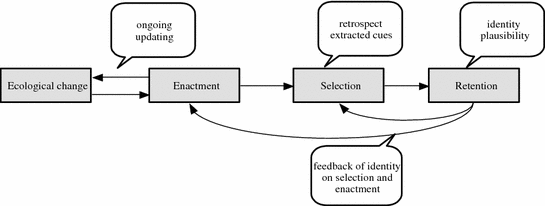
\includegraphics[width=1\linewidth]{images/Sensemaking} \end{center}

(picture from \citep{Lu_2017})

Example in business: \citep{KennethWm_2014}

\citep{Dougherty_2004}

Culture of sexual harassment (i.e., Some cultures are more prone to sexual harassment than others).

From the perspective of sensemaking theory, organizational members make sense of unexpected events through a process of
action, selection and interpretation \citep{Weick_1995}.

Organizational culture is created \textbf{not} through shared meaning, but \textbf{shared experiences through processes
sensemaking}. We might never come to a consensus, but the process of sensemaking can help us have shared experiences.

Properties of sensemaking:

\begin{itemize}
\tightlist
\item
  Identity: created through the interaction with other organizational members.
\item
  Retrospective: make sense only looking backward.
\item
  Ongoing: relate past, present, and future to make sense of an event.
\item
  Enactment: actors are part of the culture.
\item
  Extracted cues: focus their attention to parts of the environment.
\item
  Social: based on either interaction with others, or expected interaction with others.
\item
  Plausibility: seems reasonable.
\end{itemize}

Hence, sensemaking influence

\begin{itemize}
\tightlist
\item
  the acceptance of sexual harassment in an organization
\item
  responses by nonharassed members.
\end{itemize}

Sensemaking's phases:

\begin{itemize}
\tightlist
\item
  Discovery
\item
  Debriefing (e.g., humor, ridicule in case of sexual harassment)
\item
  Dispersal (e.g., return to normalcy)
\end{itemize}

men and women make of sexual harassment differently (i.e., women label more behavior as sexual harassment than men)

Practical Applications

\begin{itemize}
\tightlist
\item
  Applying Humor: humor can help members involve actively in sharing sexual harassment training, sense of community.
  But too much can also belittle victim's experience.
\item
  White men and sexual harassment: should to vilify, but assume that they want to help.
\item
  Identifying Sexual harassment: should not focus on shared meaning, but shared experience.
\item
  Responding to sexual harassment: no one-size-fit-all approach, but respect contexts of the sexual harassment.
\end{itemize}

\citep{Shenoy_Packer_2014}

First-generation immigrants are prone to microaggressions.

microaggressions are ``brief and commonplace daily verbal, behavioral, or environmental indignities, whether intentional
or unintentional, that communicate hostile, derogatory, or negative racial slights and insults''. \citep{Sue_2007}

Microagresssion exists in 3 forms:

\begin{itemize}
\tightlist
\item
  Verbal: Sarcasm
\item
  Attitudinal: Stereotypes (e.g., not fit into stereotypes, or fit into stereotypes which dismisses individual
  achievement)\\
\item
  Professional: Skepticism (e.g., microinvalidations when immigrant professionals' credentials and qualifications are
  challenged )
\end{itemize}

Sensemaking model by \citep{Weick_1995} explains how one can retrospectively make sense of past events and respond to future
events. CSM helps make sense of immigrant professional's experiences through the lenses of \textbf{power} (e.g.,
dominant-nondominant interactions).

To counter, immigrant professionals

\begin{itemize}
\item
  create another selves

  \begin{itemize}
  \tightlist
  \item
    muting/creating dual selves
  \item
    giving in
  \item
    giving up/ dissociating self
  \end{itemize}
\item
  rationalizes

  \begin{itemize}
  \tightlist
  \item
    perspective-taking
  \item
    blaming ignorance
  \item
    dismissing
  \item
    using humor
  \end{itemize}
\item
  takes ownership

  \begin{itemize}
  \tightlist
  \item
    normalizing
  \item
    appreciating cultural differences
  \item
    adapting to disparate expectation
  \end{itemize}
\end{itemize}

\citep{Williams_2017}

Communication among stakeholders in high reliability organizations (HROs)

organizational discourse: how members make sense of the tragedy by sharing.

critical team in high-hazard organization needs effective communication processes.\\
HROs are ``systems that successfully operate in environments that could produce catastrophic errors.''

3 broad themes from the grounded theory approach appear:

\begin{itemize}
\item
  Emotion

  \begin{itemize}
  \tightlist
  \item
    Some take time off to process the news.
  \item
    Some get back to work to cope with the events.
  \end{itemize}
\item
  Sensemaking (why)

  \begin{itemize}
  \item
    Debriefing process to understand what happened and learn from what happened.
  \item
    Purpose of sensemaking:

    \begin{itemize}
    \tightlist
    \item
      How could this have happened? This could happen to any other team. The fatal team was ``unlucky''.
    \item
      Why has this not happened to our team?
    \end{itemize}
  \end{itemize}
\item
  Learning (What now?)

  \begin{itemize}
  \tightlist
  \item
    Individual as well as organization(structural changes) can learn
  \end{itemize}
\end{itemize}

Making changes after a tragedy in the eyes of the crew was a routine event that officials make whenever a tragedy
happens regardless.

Staying away from blame\\
Then the question is if you did find a person's fault led to the deaths of 19 people, we can you communicate that
knowledge to facilitate learning. Moreover, the attitude of the firefighters were reluctant to changes and went back to
the basics, maybe because of this blameless culture.Hence, people might blame luck in this situation. Interestingly,
this blameless culture also facilitate group cohesion in the HROs.

A reconciliation is to recognize hindsight bias when trying to sensemaking/learning and avoid blaming.

\citep{Zanin_2019}

Athletes do not report concussion readily. They often conceal it due to cultural discourses and norms.

\textbf{Cultural narratives}

Based on \citep{Polkinghorne_1995} two-level conceptualization of narrative: actors use narrative to create social reality
and to make sense of their experiences.

Sport narrative and sensemaking:

\begin{itemize}
\item
  Sensemaking is the basis for social action.

  \begin{itemize}
  \tightlist
  \item
    Sensemaking is where meanings materialize to create identity.
  \end{itemize}
\item
  Cultural narratives help actors sensemaking by giving them a framework to understand an event.
\end{itemize}

Method: Abductive approach\\
Text Arichival Data: identify protagonist, actors, storyline, story values, and morals for each story. Then, identify
sport story archetypes

Interview \href{\%5BData:\%5D(Data:)\%7B.uri\%7D}{{[}Data:\textbackslash\textbackslash{]}(Data:)\{.uri\}} using constant comparative analysis to see how
stakeholder made sense of a concussion even and reporting behavior, then compare to the types identified in the text
archival data.

Findings:

5 narratives identified:

\begin{itemize}
\tightlist
\item
  Play-Through-Pain: enduring pain for the benefits of the team.
\item
  Big Leagues: American Dream of becoming a professional athlete through hard work and \textbf{perseverance.}
\item
  Commodification: abstract objects with financial value
\item
  Masculine Warrior: protagonist defeats an opponent through strength, toughness, bravery, violence, and
  \textbf{perseverance}
\item
  Need-for-Safety: Contemporary culture where ``athletes that seek healthcare are framed as moral and intelligent.''
\end{itemize}

Stakeholders refer to these 5 narratives to make sense of reporting behaviors.

Sensemaking use cultural sport narrative

\begin{enumerate}
\def\labelenumi{\arabic{enumi}.}
\tightlist
\item
  to extract cues: whether you have a concussion or not
\item
  construct identity: positive defense mechanism (4 over 5 narratives).
\end{enumerate}

\hypertarget{constitutive-communication-of-organizations}{%
\chapter{Constitutive Communication of Organizations}\label{constitutive-communication-of-organizations}}

\begin{itemize}
\tightlist
\item
  Social Constructionist
\item
  Structuration Theory: creation and reproduction of social systems that is based on the analysis of both structure
  and agents
\item
  little d discourse: what happen in the conversion (i.e., representation)
\item
  big D Discourse; The system of expectation you
\end{itemize}

\citep{Schoeneborn_2017}

6 premises:

\begin{itemize}
\tightlist
\item
  studies communication events (temporal and spatial dimensions).
\item
  Should be as inclusive as possible in its definition of (organizational) communication.
\item
  the co-constructed nature of (organizational) communication
\item
  who or what is acting is an open question
\item
  Communication events as unit of analysis
\item
  Equal importance of organizing (process) and organization (entity)
\end{itemize}

3 schools in CCO

\begin{itemize}
\item
  Montreal School approach: (pioneered by James R. Taylor) focus on text, speech, and linguistic forms to understand
  the their organizing properties. Organization is ``enacted through interaction and is related to processes of meaning
  negotiation''.

  \begin{itemize}
  \tightlist
  \item
    Cocretation: people talk \(\to\) interaction
  \item
    Distanciation: through time, separated, distanced from the original conversation.
  \item
    based on actor-network theory
  \end{itemize}
\item
  Four Flows approach (pioneered Robert D. McPhee): based on Giddens' structuration theory. Organization is created
  only when there are four flows:

  \begin{itemize}
  \tightlist
  \item
    Membership negotiation
  \item
    Self-structuring: constantly structuring, self here is the organization created through interaction.
  \item
    Activity coordination
  \item
    Institutional positioning (its environment)
  \end{itemize}
\item
  Social System Theory approach (pioneered by Niklas Luhmann): ``communication constitutes systems that produce the
  very elements they consist of, in a self-referential way''
\end{itemize}

Key Questions

\begin{itemize}
\tightlist
\item
  Ontological question: ``what is an organization?''
\item
  Composition problem: ``How to scale up from interaction to organization?''
\item
  Agency: ``Who ro what is able to act on behalf of the organization?''
\end{itemize}

Critiques:

\begin{itemize}
\tightlist
\item
  Bold claim that communication is organization
\item
  Too broad definition of communication.
\item
  Talk is cheap.
\end{itemize}

Emerging topics in CCO:

\begin{itemize}
\tightlist
\item
  Authority (power, domination, legitimization)
\item
  Disordering properties of communication.
\end{itemize}

\citep{Bruscella_2018}

Example of Four Flows school

terrorist organizations are communicatively constituted by the way they refer to their material as evidence to their
image, existence, and legitimacy.

organization are constructed from the following communication processes:

\begin{itemize}
\tightlist
\item
  \textbf{Self-structuring}: division of labor, rights and responsibility
\item
  \textbf{membership negotiation}: membership inclusion and exclusion criteria.
\item
  \textbf{activity coordination}: mutual adjustments of action
\item
  \textbf{institutional position}: defining the boundaries of the organization
\end{itemize}

Question of agency:

\begin{itemize}
\tightlist
\item
  Four Flows theory define agency as human unique ability to make their own choice, while the Montreal School define
  agency as the ability to make a difference (e.g., humans or nonhumans). Hence, this paper included materials into
  the Four Flow Theory as the
\end{itemize}

Materials (or economics) can give inference about legitimacy, permanence, and credibility.

Hidden organization challenged the assumption of visibility from the Montreal school.

ISIL used a propaganda magazine (Dabiq) - communication- to illustrate their image and identity to its members

three communication strategies in their institutional positioning communication:

\begin{enumerate}
\def\labelenumi{(\arabic{enumi})}
\tightlist
\item
  instantiation: give artifacts to explain arguments.
\item
  cooptation: ``adoption of a rival's messaging for a purpose different from its original use.''
\item
  intertextual allusion: " a language form in which an association with a sacred, mythic, or origin text is insinuated
  by way of communication shortcuts."
\end{enumerate}

\citep{Koschmann_2015}

\citep{Knuf_1993} defines organizational rituals ``in terms of their formality, sacredness, irrationality, and aesthetics.''

``what rituals do is make present an authoritative text, and how they do this is through the attribution and
appropriation of possessive constitution.''

Organizations is an ``abstract textual representations of power and legitimacy that are manifest in practice.'' Hence,
Certain kinds of interactions (i.e., organizational rituals) create organization.

Authoritative text ``portrays the structure of the organization in ways that specify roles, duties, values, activities,
outcomes, and the like, while also explaining relations of power and legitimacy''.

Specifically rituals found in this study:

\begin{itemize}
\tightlist
\item
  The opening
\item
  Sharing the critter: appreciation
\item
  Card signing
\item
  Spanish lesson
\item
  Reciting the mission statement
\item
  Moment of silence
\end{itemize}

Ritual Agency

\begin{itemize}
\tightlist
\item
  Rituals remind
\item
  Rituals discipline: instill or and constraining behavior.
\end{itemize}

Inclusion is authoritative text which constructs their organization. Hence, rituals are practices that shows inclusion.

\citep{Cooren_2015}

ventriloquism denotes ``action through which someone or something makes someone or something else say or do things''.
\citep{Cooren_2010}. For example, a layer is a ventriloquist while a contract is a dummy or figure.

\begin{itemize}
\tightlist
\item
  Ventriloquism is bi-directionality.
\item
  Figure or dummy can increase ventriloquist's authority
\item
  communication becomes the means through which some aspects of the world contradict or align themselves with other
  aspects of the world. From a ventriloqual point of view, the world is not a place where communication is detached
  from the things that matter."
\end{itemize}

\citep{Trittin_2015}

Diversity in organization cannot be superficially achieved by pre-defined unchanged characteristics (i.e., gender).
Hence, in this study, authors defined diversity as ``the plurality of''voices," that is, the range of individual opinions
and societal discourses that get expressed and can find resonance in organizational settings."

\begin{itemize}
\tightlist
\item
  One can have many voices, and one voice can be manifested by multiple individuals.
\end{itemize}

Instrumental Perspectives on Diversity Management:

\begin{itemize}
\tightlist
\item
  Traditionally, diversity was thought as the difference between individuals, where communication (unidirectional,
  controllable, and linear process of information transmission) is a moderator of diversity on performance.
\item
  Later, diversity as diversified value orientation \citep{Eastman_2003}, work styles \citep{Shelton_2002}, education background
  \citep{Kearney_2009}.
\end{itemize}

Critical Perspectives on Diversity Management:

\begin{itemize}
\tightlist
\item
  Radical -critical: you can't manage diversity in organizational settings.
\item
  Constructive critical: instrumental approach can be both economically successful and socially just.
\end{itemize}

This paper follows the Montreal school of thought.

\hypertarget{socialization}{%
\chapter{Socialization}\label{socialization}}

\citep{Kramer_2011}

According to \citep{Van_Maanen_1979}, socialization is defined as ``the process by which an individual acquires the social
knowledge and skills necessary to assume an organizational role.''

Levels of analysis:

\begin{itemize}
\item
  Single Organization Voluntary Socialization: Individual voluntary membership:

  \begin{itemize}
  \tightlist
  \item
    Membership negotiation
  \end{itemize}
\item
  How individuals' multiple group memberships interact to affect their socialization
\item
  how the multiple group memberships of other influence the socialization process of an individual.
\end{itemize}

Personally, I'd not define the way the author structured the research as levels of analysis because they are all at the
individual level.

Personalization: new members try to change aspects of the organization to fit their needs.

Communication:

\begin{itemize}
\tightlist
\item
  Reconnaissance communication: is when prospective members to obtain info about the organization.
\end{itemize}

Membership statuses are fluid, and transitory, overlapping

\citep{Myers_2010}

Vocational Anticipatory Socialization (VAS) tries to predict individual's interests and their career pursuit using
socialization theory.

Factors affecting the number of students choosing STEM field:

\begin{itemize}
\tightlist
\item
  Social factors
\item
  Personal interest
\end{itemize}

Sources of VAS:

\begin{itemize}
\tightlist
\item
  Family members: especially parents, socialize their children to various notions of jobs and careers.
\item
  Educational Institution: learn about power and social skills which later affects career choice.
\item
  Part-time jobs: good start for students to be socialize into the career network.
\item
  Peers: influence expectation of a future career.
\item
  Media: socialize value and expectations about careers.
\end{itemize}

Career Development Models :

\begin{enumerate}
\def\labelenumi{\arabic{enumi}.}
\tightlist
\item
  life-space model \citep{Vondracek_2019}:
\end{enumerate}

\begin{itemize}
\tightlist
\item
  Physiological factor (e.g., country of origin, genetics).
\item
  Psychological characteristics: (e.g., self-concept, development of intelligence, values, needs, interests, ability,
  aptitudes).
\item
  Socioeconomic environments
\end{itemize}

5 life stages:

\begin{itemize}
\tightlist
\item
  Growth (0-14)
\item
  Exploration (15-24)
\item
  Establishment (25-44)
\item
  Maintenance (45-64)
\item
  Decline (after 65)
\end{itemize}

9 roles:

\begin{itemize}
\tightlist
\item
  Child
\item
  Leisurite
\item
  Citizen
\item
  Worker
\item
  Pensioner
\item
  Spouse
\item
  Homemaker
\item
  Parent
\end{itemize}

\begin{enumerate}
\def\labelenumi{\arabic{enumi}.}
\setcounter{enumi}{1}
\tightlist
\item
  Social-cognitive career choice model: \citep{Lent_1994}
\end{enumerate}

Self-efficacy mediate the relationship between ability and interests. A feedback loop is created once a person form
career choice goals from self-efficacy and outcome expectations

VAS differs from these two models that it studies the socializing agents.

Found both gender (even though students deny such an effect, but they admit the social effects of others) and culture
and Socioeconomic Status affect career choice. \textbf{Experience} (exposure, job shadowing), \textbf{personal factors} (i.e.,
individual-level variables) also affect career choice (consistent with social-cognitive career).

VAS Messages:

\begin{itemize}
\tightlist
\item
  Value (e.g., family)
\item
  Expectation (e.g., self expectation of career)
\item
  Prescription (e.g., career choice should based on talents, interests,career's prestige and income potential )
\item
  Opportunity (e.g., take careers that are under pursued, hence more job opportunities).
\item
  Description (e.g., t job-specific environments, tasks, satisfaction, and required knowledge)
\end{itemize}

Check \citep[pp.107]{Myers_2010} for framework of VAS in STEM.

\citep{smith2012}:

Master narratives should be understood in tandem with personal narratives. \citep[pp.209]{tannen2008} defines master
narrative as ``a culture-wide ideology that shapes the big-N Narrative.'' In contrast with small-n where it personal
stories and experiences can be found, Big-N Narratives are those that create a background for small-n narratives.

Retirement is a socialization process of the master narrative of aging and the American dream (e.g., success, and
freedom - financial, responsibility).

Groups:

\begin{itemize}
\tightlist
\item
  Anticipatory group
\item
  Early work life
\item
  Preretirement
\item
  Retiree
\end{itemize}

Fractures of the master narrative:

\begin{itemize}
\tightlist
\item
  Freedom/routine fracture: they still want some work (structure), to stay active and productive members of society
\item
  Individual responsibility/universal expectations fracture: individual is responsible for one's happiness.
\end{itemize}

\citep{ferguson2017}

\citep{jablin_1987} defines socialization as a ``developmental unending process which can be broken up into three stages:
\textbf{anticipatory, assimilation, and exit}.''

assimilation with others African American. Later on, in college, the author tried closet his identity and desire.

\citep{Gibson_2000}

Organizational Assimilation Processes: blue-collar usually seen as routine and repetitive, tedious hence less creative,
less motivation.

Consent that they need money and later on assimilate into the organizations. Formally, \citep[pp.712]{jablin_1987} defines
organizational assimilation as ``those ongoing behavioral and cognitive processes by which individuals join, become
integrated into, and exit organizations.''

Stages of socialization:

\begin{itemize}
\tightlist
\item
  Anticipatory socialization
\item
  encounter
\item
  metamorphosis: accepted into the organization, and consistent with the organization's expectation. (outgroup \(\to\)
  ingroup)
\end{itemize}

Concertive control is ``a form of organizational control that emerges in accordance with the dominate ideologies in the
organization, usually managerial-based.''

Workers construct hard-working identity and are proud of it.

\hypertarget{worklife}{%
\chapter{Worklife}\label{worklife}}

\citep{Langellier_2006} Somebody's got to pick eggs - family storytelling

traditional allocation by generation and gender.

Children don't typically question their tasks. But family stroytelling ``can be understood as a struggle over meanings
and material resources for family, work, and nation.''

\citep{Kirby_2002}

using \citep{gidden_1984} Structuration Theory. Having a policy doesn't mean it will be enacted or practiced.

Work-Family Policy Implementation: Supervisors discourage employees to take work-family benefits

Coworker Communication: people who don't use these policies feel unjust (i.e., more work for them). Coworkers reinforce
or undermine work-family policy implementation. Employees feel resentment for those who take the leaves (there is a
sense of preferential treatment, perception of inequity).

Meritocracy plays a big role in the inequity perception.

\citep{Wieland_2011}

understand work and life ``as a struggle through which control and resistance are accomplished as various meanings of
work are negotiated.''

This study see work/life issues under the dialectical view of \textbf{control} and \textbf{resistance} (where it might not be an
individual deviance, but unobtrusive act) at Swedish organization.

2 types of ``goods'':

\begin{itemize}
\item
  well-being

  \begin{itemize}
  \item
    is an end in itself
  \item
    is a means to an organizational end: instrumental way to achieve delivering
  \end{itemize}
\item
  delivering
\end{itemize}

``balance'' is not the solution as well-being is considered a means to an organizational end, which is parallel to
delivering.

\citep{D_Enbeau_2015}

Women caught in between the Western and non-Western cultures in the context of work life.

Feminine-typed careers (e.g., nursing, teaching, social work) offer lower wages, little room for growth, and long
working hours

Equity-Difference Tension:

\begin{itemize}
\tightlist
\item
  Women's interpretation of religion (e.g., Muslim) to overcome their identity role.
\item
  Solution: Reframing Gender Difference as Gender Complementary: Women and men help each other in work-life.
\end{itemize}

Modernity-tradition Tension:

\begin{itemize}
\tightlist
\item
  Traditional maternal roles: should not sacrifice work for mother role
\item
  Patriarchal family norms: women still honor the patriarchal role by choosing approved role set by her father.
\item
  Solution: Professional and familial success: you are not successful if you can't share it with your family.
\end{itemize}

Individual-Collective Tension:

\begin{itemize}
\tightlist
\item
  Women in the group try to change gender norms
\item
  They aren't sure if they should adhere to cultural gender norms
\item
  Solution: cultural pride was interpreted as the reason for women to work to change collective gender norms.
\end{itemize}

\citep{Banghart_2018}

Boundaries can exist among:

\begin{itemize}
\tightlist
\item
  private/personal
\item
  work/professional
\item
  public/political
\end{itemize}

However, these boundaries can be permeable or rigid

Increased formal social media policies (SMPs) - ``when, where and how employees should engage with and communicate
through social media.'' \citep{Vaast_2013}

Boundary logics ``embody the implicit and explicit organizational assumptions about the permeability or rigidity of
boundaries between personal and organizational domains.''

Companies can also use

\begin{itemize}
\tightlist
\item
  \emph{evasive boundary logic}: ambiguity of boundaries serve to provide a wide range of interpretation. Hence, different
  employees have different definition of boundaries.
\item
  \emph{distinct boundary logic}: how employees should conduct their social presence, where all boundaries are rigid, and
  segmentable.
\item
  \emph{invasive boundary logic}: integration approach to boundary, boundaries are permeable (e.g., any messages on social
  media can reflect back on the company).
\item
  \emph{contradictory boundary logic}: permeable and rigid at the same time.
\end{itemize}

Companies with general and unspecified directives can confuse and infringe upon employee rights.

\hypertarget{emotions-and-organizing}{%
\chapter{Emotions and Organizing}\label{emotions-and-organizing}}

\citep{Mumby_1992}

bounded rationality was developed around patriarchal modes of
organizing.

\begin{itemize}
\item
  Deconstruction benefits feminism:

  \begin{itemize}
  \item
    ``exposes the political nature of categories'' (e.g., nature, and
    gender)
  \item
    exposes oppressive system of hierarchy by challenging
    dichotomous thinking.
  \item
    helps rethinking power and identity
  \end{itemize}
\item
  Bounded emotionality was created to challenge bounded rationality,
  but not to be its opposite.
\item
  bounded rationality grounded in ``satisficing''
\item
  four premises of feminist view on bounded rationality:

  \begin{itemize}
  \item
    the centrality of the cognitive metaphor
  \item
    the emphasis on a mind-body dualism
  \item
    the devaluing of physical labor
  \item
    the treatment of emotion as a form a labor
  \end{itemize}
\item
  \citep{hochschild2012} defined emotional labor as ``the way individuals
  change or manage emotions to make them appropriate or consistent
  with a situation, a role or an expected organizational behavior.''

  \begin{itemize}
  \item
    emotional labor becomes a commodity for organization to achieve
    its goal.
  \item
    \emph{However, I disagree with this idea because people can be
    happier even when they fake smile.}
  \end{itemize}
\item
  bounded emotionality is ``an alternative mode of organizing in which
  nurturance, caring, community, supportiveness, and interrelatedness
  are fused with individual responsibility to shape organizational
  experience.''
\item
  bounded emotionality also tries to reduce emotional labor and
  gendered divisions of labor (e.g., women can express work feeling).
\end{itemize}

After reading this piece, I was still not convinced that bounded
rationality is rooted in patriarchy. Authors argued that since previous
researchers are so embedded in the bureaucratization of organization
that they don't realize power-knowledge relationship.

\citep{Kramer_2002}

Emotion management in organization:

\begin{itemize}
\tightlist
\item
  at the center is ``professionalism''
\item
  both positive and negative emotions, need to be display in
  appropriate ways
\item
  the appropriate way of displaying negative emotions is masking them.
\item
  using emotions to help others, not for oneself.
\end{itemize}

Emotions are typically understood in terms of expectancy violation

Organizations are indoctrinated to favor positive emotions.

\citep{Rivera_2014}

Using the framework of emotional taint to understand dirty works (e.g.,
border patrol).

Sometimes dirty work does not exclusively relate to physical or danger
activities but include those social taint (e.g., exotic dancers)

Emotional labor ``includes outward performances of emotions'' (e.g.,
smiling, yelling, showing no emotions) is socially constructed.

Sensemaking of identities, dirty work by using past works.

This line of work (e.g., law enforcement) prefers more masculine
emotional labor (e.g., use of force continuum)

Stoicism is a form of emotional labor. Emotional labor is dirty work.

Criticism of feminine care work and compassion, which is parallel to
men's struggle with perception of sexuality when they act caring

Making sense of taint by expressing tensions:

\begin{itemize}
\tightlist
\item
  Agents are at the crossroad of society's view of their work (e.g.,
  positive and negative)
\item
  They have to switch between 2 types of emotional labor (e.g.,
  stoicism and compassion)
\end{itemize}

Emotional Taint Management:

\begin{itemize}
\tightlist
\item
  Strategically engage in different emotions
\end{itemize}

\citep{Jia_2016}

\begin{itemize}
\item
  emotions are expressed through communication
\item
  supervisor nonverbal immediacy influences subordinates' emotional
  experience (e.g., emotion work, and perceived emotional support)
\item
  Emotional response theory: people respond to external environmental
  stimuli (e.g., emotion inducing factor - nonverbal immediacy by
  supervisors).
\item
  According to \citep{Mehrabian_1967}, nonverbal immediacy are
  ``communicative behaviors used to enhance physical or psychological
  closeness and reduce interpersonal distance'' (e.g., touching,
  nodding, smiling).
\item
  \citep{titsworth2010} defined three dimensions of student emotional
  experience in response to teacher communication:

  \begin{itemize}
  \item
    Emotional valance: positive/negative reactions
  \item
    Emotion work: intentional management of emotional expression,
    could lead to emotional exhaustion or burnout
  \item
    Emotional support: perception of receiving emotional support
  \end{itemize}
\item
  ``Supervisor NI will be positively correlated with subordinates'
  perceptions of received emotional support from the supervisor''
\item
  According to \citep{RUBIN_1988}, based on goal-oriented behaviors, there
  are six motives for interpersonal communication:

  \begin{itemize}
  \item
    relationally oriented motives (used to facilitate positive
    encounters)

    \begin{itemize}
    \item
      pleasure
    \item
      affection
    \item
      relaxation
    \item
      inclusion
    \end{itemize}
  \item
    personal-influence motives (used to manage interaction)

    \begin{itemize}
    \item
      escape
    \item
      control
    \end{itemize}
  \end{itemize}
\item
  Supervisor NI enhance employees' received emotional support, and
  reduce employees' engagement in emotion work
\end{itemize}

\hypertarget{identity}{%
\chapter{Identity}\label{identity}}

\citep{Tracy_2005}.

\begin{itemize}
\item
  The self is "a product or an effect of competing, fragmentary,a nd
  contradictory discourse \citep{Tracy_2005}
\item
  Since we spend most of our lives at work, identities are now
  typically based on organizational and workgroups.
\item
  People performing ``dirty'' work typically perform and perceive
  different selves (real vs.~fake)
\item
  There are no real or fake, but ``crystallized''

  \begin{itemize}
  \tightlist
  \item
    multi-dimension, (multi facets, and complex).
  \end{itemize}
\item
  Constituted Self: one is a thinking, feeling subject, and social
  agent
\item
  Deep vs.~surface acting: both are separated from the ``real'' self

  \begin{itemize}
  \item
    deep acting = change how they feel
  \item
    surface acting = outward expression changed without changing
    internal feeling
  \end{itemize}
\item
  Emotional labor creates emotive dissonance/discomfort
\item
  but we should conceptualize self as single self.
\item
  under the power discourse, organization prefers the dichotomized
  category of self.
\item
  should not call real, but ``preferred'' self
\item
  crystallization is ``enacted in local/temporal moments.''
\end{itemize}

\citep{Stephens_2013}

\begin{itemize}
\item
  Using social identity theory, \citep{Stephens_2013} hypothesize and find
  that people's identification with a message source (HIT- health
  information technologies) mediates the effect of social media on
  outcomes.
\item
  According to social identity theory (SIT), one of the aspect of
  identity is affiliated with organization.

  \begin{itemize}
  \tightlist
  \item
    Organizational identification increase affect involvement,
    satisfaction and organizational commitment \citep{Ashforth_2008}
  \end{itemize}
\item
  HIT can be either

  \begin{itemize}
  \item
    social function: social media
  \item
    information source (e-mail and websites)
  \end{itemize}
\end{itemize}

\citep{Meisenbach_2014}

\begin{itemize}
\tightlist
\item
  In the context of voluntary work, identities are (re)created via
  communicative behaviors.
\item
  Voluntary works are ways to enact participants' nested identities
  (e.g., choir, music and family identities).
\end{itemize}

\citep{Compton_2016}

\begin{itemize}
\item
  Applying CTI (communication theory of identity) to the context of
  organizational employees managing their sexual identity.
\item
  Identity gap exists between

  \begin{itemize}
  \item
    relational identity and enacted identity,
  \item
    relation and communal identity
  \end{itemize}
\item
  Policy text is different from policy talk

  \begin{itemize}
  \tightlist
  \item
    Policy and practices can be different.
  \end{itemize}
\item
  participants receive mixed messages:

  \begin{itemize}
  \item
    supportive
  \item
    discriminatory
  \end{itemize}
\item
  don't scarify your life for your job (you should check your policy
  first)
\end{itemize}

\hypertarget{power-privilege}{%
\chapter{Power \& Privilege}\label{power-privilege}}

organizational power negotiated with individual power to create an
enmeshed privileges that we see

\citep{de_la_Garza_2020}

\begin{itemize}
\tightlist
\item
  Hashtag is just a show for public solidarity without real
  substantive changes
\item
  we must shed light on marginalized groups, not only celebrity voices
\item
  shouldn't normalize the \#MeToo, but it should serve to put
  discomfort on perpetrators.
\end{itemize}

\citep{Gan_2020}

\begin{itemize}
\tightlist
\item
  Since university employees are constantly silent, they feel that
  they are belittle, and their efforts are futile.
\item
  Just like Plato's story of the cave, the perceived reality are only
  reflection of manipulated images of the truth, university with
  organizational power only see what they want to see. If it allows
  voices of its employees to be heard, the reality could be different
  or even improved.
\end{itemize}

\citep{D_Enbeau_2013}

\begin{itemize}
\item
  two paradoxes in practice:

  \begin{itemize}
  \item
    paradox of consistency: expected consistency between
    organizational philosophy and practice, but this alignment
    inhibits empowerment.

    \begin{itemize}
    \item
      Solution:

      \begin{itemize}
      \item
        distinction between meaningful and non-meaningful work
      \item
        distinction between work and non-work.
      \end{itemize}
    \end{itemize}
  \item
    paradox of transparency: ``employees' desire for clarity of
    empowerment meanings in client interactions, goals,a nd
    outcomes.''

    \begin{itemize}
    \tightlist
    \item
      Solutions: staff has alternative meanings of empowerment.
    \end{itemize}
  \end{itemize}
\end{itemize}

\citep{Kantola_2014}

\begin{itemize}
\item
  Mediatization of corporate management
\item
  Media has become tools of power of corporate power within flexible
  capitalism.
\item
  Mediatization of power:

  \begin{itemize}
  \item
    mediatization has 4 processes \citep{Schulz_2004}:

    \begin{itemize}
    \item
      extension: communication extends the communication
      capacities of the CEO
    \item
      substitution: replace the controlling hierarchies of
      supervision
    \item
      amalgamation: amalgamated with the exercise of power in
      corporate capitalism
    \item
      accommodation: to media by planning their communication
      strategies.
    \end{itemize}
  \item
    media prospers under the structures of power
  \item
    mediatization of CEOs:

    \begin{itemize}
    \item
      changes in the media
    \item
      changes in corporate capitalism
    \end{itemize}
  \end{itemize}
\item
  Media Logic in Corporate Life

  \begin{itemize}
  \tightlist
  \item
    media has gained CEO's coverage in the early twentieth century
    \citep[pp.~31]{Kantola_2014}
  \end{itemize}
\item
  Mediatization theory: media shapes and frames the processes and
  discourse (conversation) of political communication and the society.
\item
  industrial capitalism to flexible post-Fordist capitalism

  \begin{itemize}
  \tightlist
  \item
    But others called from managerial capitalism to investor
    capitalism. (see Khurana).
  \end{itemize}
\item
  Mediatization and celebritization are intertwined
\item
  CEOs use affective appeal to get affective power of the populace.

  \begin{itemize}
  \tightlist
  \item
    They use celebrity-making tactics.
  \end{itemize}
\end{itemize}

\textbf{The web-of-power-exploring communication and social class}

\begin{itemize}
\item
  Social class is about power
\item
  Power (Mumby, 1998):

  \begin{itemize}
  \item
    Systems rationality perspective: struggle over scarce resources'
    distribution
  \item
    Interpretive perspective; centered in communication (how people
    socially constructed shared meanings).
  \item
    Critical perspective: power = domination where ruling class
    dominates the working class.
  \item
    Post-modern perspectives: power = fragmented and individual. And
    the focus is on discourse.

    \begin{itemize}
    \tightlist
    \item
      Poststructuralism: modified vision of postmodernism, where
      society is structured through discourse.
    \end{itemize}
  \item
    Feminism: patriarchy is power.
  \item
    Power can also be viewed in relation to social class, age, race,
    gender, sexuality, and ability
  \end{itemize}
\item
  Social class:

  \begin{itemize}
  \item
    physically unmarked, but communicatively marked
  \item
    inherently unstable in meaning, but also stable as the same
    populations remain in the same social class strata
  \item
    represents ongoing struggle
  \item
    the web-of-power is weaved into social class
  \item
    Social class talk:

    \begin{itemize}
    \tightlist
    \item
      text class (transcend body impediment) vs body class
    \end{itemize}
  \end{itemize}
\end{itemize}

\hypertarget{tension-contradiction-and-paradox}{%
\chapter{Tension, Contradiction, and Paradox}\label{tension-contradiction-and-paradox}}

\citep{Wood_1983}

Difficulties experienced by women in American labor force are studied
under:

\begin{itemize}
\item
  societal research: sex-role stereotypes
\item
  organizational perspective: organizational structures that are
  barriers
\item
  individualistic research: based on personalities and activities that
  make it difficult for women to be professionals.
\end{itemize}

Paradox, mystification, and the double-bind

Responses that Perpetuate the Double-binding Pattern

\begin{itemize}
\item
  acceptance
\item
  counter-disqualification
\item
  withdrawal
\end{itemize}

Double-binds composed of:

\begin{itemize}
\item
  type of relational situation: complementary relationship with
  unbalanced power structure
\item
  paradox-creating communication: mixed messages
\item
  responses (by person with less power) that solidify the pattern
\end{itemize}

Mystification: ``the symbolic processes whereby one socio-economic group
misrepresents action in order to maintain its hegemony over another
socio-economic group.''

\begin{itemize}
\tightlist
\item
  mystification is a manifestation of bullying
\end{itemize}

In Western culture, women's stereotypical roles:

\begin{itemize}
\item
  sex object,
\item
  pet
\item
  mother
\item
  iron maiden
\end{itemize}

Professional are thought of as:

\begin{itemize}
\item
  rationality
\item
  power
\item
  decisiveness
\item
  activity
\item
  objectivity
\item
  toughness
\end{itemize}

Paradoxes in organizations:

\begin{itemize}
\item
  powerlessness
\item
  marginality and minority

  \begin{itemize}
  \item
    success can be attributed to ease of task, perseverance, not
    competence.
  \item
    lone women status
  \end{itemize}
\item
  self-definition
\item
  affirmative action
\item
  training programs
\item
  networks and mentor relationships
\end{itemize}

Responses to paradox:

\begin{itemize}
\item
  responses that perpetuate the situation

  \begin{itemize}
  \item
    acceptance
  \item
    counter-disqualification
  \item
    withdrawal
  \end{itemize}
\item
  responses that redefine the situation

  \begin{itemize}
  \item
    interpret in a fresh frame-of-reference
  \item
    redirection
  \item
    confrontation
  \end{itemize}
\item
  responses that transcend the situation
\end{itemize}

\citep{Trethewey_2004}

\begin{itemize}
\item
  reframe organizational tension:

  \begin{itemize}
  \item
    irrationality (e.g., paradox, contradiction, irony) is normal
  \item
    irrationalities are gendered
  \item
    irrationality is an applied concern
  \end{itemize}
\end{itemize}

\citep{Way_2019}

\begin{itemize}
\item
  Youth Crew context
\item
  tension between youths and adults in summer camp
\item
  tension is a ``\,`feeling state,' specifically the discomfort
  experienced by organizational members when they encounter
  organizational practices and structures that are contradictory or
  paradoxical.'' \citep{Putnam_2016}
\item
  Youth work is just preparatory experience for future work.
\item
  Paradoxes

  \begin{itemize}
  \item
    Providing vs.~discounting oneself as worker
  \item
    demanding confidence vs.~orchestrating uncertainty
  \item
    playing along vs.~being playful
  \end{itemize}
\end{itemize}

Acting to Alter Privilege by Maintaining the Structural-Performative
Paradox by Sonja K. Foss

\begin{itemize}
\item
  paradoxical perspectives on privilege---the structural and the
  performative
\item
  paradoxes of privileges:

  \begin{itemize}
  \item
    dispersal-divestment: disperse privilege, but also divest it.
  \item
    alteration-reproduction: when you try to combat prvilidge, it
    backfires
  \end{itemize}
\end{itemize}

\hypertarget{organizational-change}{%
\chapter{Organizational Change}\label{organizational-change}}

This section is a summary and critique of ``Organizational Change'' by \citep{Lewis_2019}

Organizations are ``socially constructed largely through the communicative interactions of internal and external
stakeholders''.\\
Stakeholders are those ``who have a stake in an organization's process and or outputs''.\\
Ripple effects are ``the impacts that organizational actions and presence bring to stakeholders within and surrounding
the organization''.

Even though the fad nature of society values change and associate with positive terms, compared to negative connotations
of stability. However, changes does not equate good.\\
Triggers for organizational changes:\\
(external)

\begin{itemize}
\tightlist
\item
  Legal requirements
\item
  Stakeholders
\item
  Current business, societal, environmental trends
\item
  Technologies
\item
  Availability of financial resources
\item
  Alteration of relationship, powers, and global economy.
\end{itemize}

(internal)

\begin{itemize}
\tightlist
\item
  innovation
\item
  serendipity
\end{itemize}

Communication is key for changes because not until stakeholders recognize and communicate change that it materializes in
an organization.

Sensemaking is both ``authoring'' and interpretation \citep{Lewis_2019}. Communication among stakeholders is at the heart of
change processes in organizations because of this highly social process of making sense of what is going on and
``spinning it into narratives and theories of the world around us.'' \citep{Lewis_2019}.

Costs of change:

\begin{itemize}
\item
  Financial
\item
  Opportunities:

  \begin{itemize}
  \tightlist
  \item
    Lost productivity
  \item
    Lost time in training works
  \item
    Workflow
  \item
    Loss of high value stakeholders.
  \end{itemize}
\item
  Miscommunication: Confusion, fatigue.
\item
  Brand
\end{itemize}

\citep[p.10]{Zorn_1999} define organizational change as ``any alteration or modification of organizational structures or
processes.''

Process of change:

\begin{itemize}
\tightlist
\item
  Innovation: (creating) idea generation
\item
  Adoption: (deciding) formal decision by leaders
\item
  Diffusion: (sharing) sharing of ideas.
\item
  Implementation: ``the translation of any tool or technique, process, or method of doing, from knowledge to practice.''
  \citep{Tornatzky_1982}
\item
  Discontinuation: later, changes will become obsolete and a new cycle begins.
\end{itemize}

Communication is at the heart of all of these phases.

For relationships between innovation, diffusion, adoption, and implementation, check \citep[pp.~35]{Lewis_2019}

Types of Organizational change:

\begin{itemize}
\item
  Planned vs.~unplanned changes
\item
  Objects that are changed (e.g., technologies, programs, policies, processes, personal). But not good in practice due
  to blur lines among these objects.
\item
  Discursive change (i.e., new label for old things to fake change) vs.~material change (i.e., real changes in terms
  of operations, practices, relationships, decision-making) \citep[pp.10]{Zorn_1999}
\item
  Size and scope of change \citep{Bartunek_1987} (however, size and scope can be subjective):

  \begin{itemize}
  \item
    First-order changes: small
  \item
    Second-order changes: large transformations, disruptive
  \item
    Third-order changes: continuous change.
  \end{itemize}
\end{itemize}

Combinations of these types of organizational change can be viewed in \citep[pp.~42]{Lewis_2019}

Complexity of change within organizations:

\begin{itemize}
\item
  Interdependence: " The degree to which stakeholders impact the lives of other stakeholders as they engage change."
  \citep{Lewis_2019}

  \begin{itemize}
  \tightlist
  \item
    Sequential Interdependence: Stakeholders affect one another in sequence (e.g., assembly line).
  \item
    Reciprocal interdependence: stakeholder's input are another stakeholder's outputs and vice versa. (e..g,
    co-authors).
  \end{itemize}
\item
  organizational structures:

  \begin{itemize}
  \item
    Structures: are rules and resources (e.g., information, status, organizational beliefs, ) that create
    organizational practices
  \item
    Types of Structures:

    \begin{itemize}
    \tightlist
    \item
      Decision-making patterns
    \item
      Decision-making processes
    \item
      Ladders of authority
    \item
      Role relationships
    \item
      Information-sharing norms
    \item
      Communication networks
    \item
      Reward system
    \end{itemize}
  \end{itemize}
\item
  Politics
\end{itemize}

Key processes in communication of planned change

\begin{itemize}
\tightlist
\item
  Dissemination of information
\item
  Soliciting input
\item
  Socialization
\end{itemize}

Types of communication in change implementation

\begin{itemize}
\tightlist
\item
  Formal Communication
\item
  Informal Communication: ``includes spontaneous interactions of stakeholders with each other, with implementers, and
  with non-stakeholders.''
\end{itemize}

change requires the following resources:

\begin{itemize}
\tightlist
\item
  Physical
\item
  Financial
\item
  Emotional
\item
  Political
\item
  Rhetorical and discursive
\end{itemize}

\textbf{Processes} are ``sets of actions designed and directed toward some desired outcome''

\textbf{Communication processes} consist of

\begin{itemize}
\tightlist
\item
  interaction
\item
  discourse
\item
  interpretation
\end{itemize}

Communication processes in the context of change:

\begin{itemize}
\item
  information dissemination: is used to reduce uncertainty

  \begin{itemize}
  \item
    Uncertainty is defined as ``a lack of information or as confusion related to many available possible
    interpretations of events or objects.''
  \item
    Change comes with \citep{Bordia_2003}:

    \begin{itemize}
    \item
      Strategic Uncertainty (e.g., relation to the external environment)
    \item
      Structural Uncertainty (e.g., culture)
    \item
      Job-related Uncertainty
    \end{itemize}
  \item
    However, uncertainty is not always bad, or arises from lack of information. \textbf{Equivocality} (i.e., ambiguous
    meanings and overwhelming available interpretations of events or objects) can be troublesome too.
  \item
    Solution offered by \citep{Weick_2015} that focuses on processes of interpretation construction

    \begin{itemize}
    \item
      arguing
    \item
      expecting
    \item
      committing
    \item
      manipulating
    \end{itemize}
  \item
    Knowledge in organizational change:

    \begin{itemize}
    \tightlist
    \item
      \citep{Kuhn_2008} defines \textbf{knowledge} (a noun) as stable facts, objects, and dispositions, and \textbf{knowing} (a
      verb): an active and ongoing accomplishment of problem solving.
    \end{itemize}
  \end{itemize}
\item
  \textbf{soliciting}

  \begin{itemize}
  \item
    input from stakeholder can:

    \begin{itemize}
    \item
      lower resistance to change
    \item
      increase satisfaction of participants
    \item
      increase stakeholders' feelings of control
    \item
      reduce uncertainty about change.
    \end{itemize}
  \item
    to maximize input, we can adopt \textbf{USER}:

    \begin{itemize}
    \item
      \textbf{Use} input as a resource in the decision-making process
    \item
      \textbf{Systematically} collect input
    \item
      \textbf{Evaluate} the the process
    \item
      \textbf{Rigorously} examine collected input
    \end{itemize}
  \item
    voice can be

    \begin{itemize}
    \item
      full voice: actual, meaningful engagements by stakeholders
    \item
      limited voice: when changes are easily made or aligned with the implementer' idea.
    \item
      faux voice: channels to vent, but not material changes
    \end{itemize}
  \item
    implementer can treat stakeholder participation as:

    \begin{itemize}
    \item
      symbol
    \item
      resource
    \end{itemize}
  \item
    Authenticity and trust perception influences on the likelihood and how stakeholders will give inputs.
  \end{itemize}
\end{itemize}

\begin{longtable}[]{@{}ll@{}}
\caption{\citep[pp.75]{Lewis_2019}}\tabularnewline
\toprule
\begin{minipage}[b]{(\columnwidth - 1\tabcolsep) * \real{0.58}}\raggedright
Direct (individuals represent themselves)\strut
\end{minipage} & \begin{minipage}[b]{(\columnwidth - 1\tabcolsep) * \real{0.42}}\raggedright
Indirect (representative for a group)\strut
\end{minipage}\tabularnewline
\midrule
\endfirsthead
\toprule
\begin{minipage}[b]{(\columnwidth - 1\tabcolsep) * \real{0.58}}\raggedright
Direct (individuals represent themselves)\strut
\end{minipage} & \begin{minipage}[b]{(\columnwidth - 1\tabcolsep) * \real{0.42}}\raggedright
Indirect (representative for a group)\strut
\end{minipage}\tabularnewline
\midrule
\endhead
\begin{minipage}[t]{(\columnwidth - 1\tabcolsep) * \real{0.58}}\raggedright
Forced (providers are required to participate)\strut
\end{minipage} & \begin{minipage}[t]{(\columnwidth - 1\tabcolsep) * \real{0.42}}\raggedright
Voluntary (individuals offer freely)\strut
\end{minipage}\tabularnewline
\begin{minipage}[t]{(\columnwidth - 1\tabcolsep) * \real{0.58}}\raggedright
Formal (committees or task forces)\strut
\end{minipage} & \begin{minipage}[t]{(\columnwidth - 1\tabcolsep) * \real{0.42}}\raggedright
Informal (water-cooler moments)\strut
\end{minipage}\tabularnewline
\begin{minipage}[t]{(\columnwidth - 1\tabcolsep) * \real{0.58}}\raggedright
publicly and identified (open staff meeting)\strut
\end{minipage} & \begin{minipage}[t]{(\columnwidth - 1\tabcolsep) * \real{0.42}}\raggedright
Privately or anonymous (privately to a
consultant)\strut
\end{minipage}\tabularnewline
\begin{minipage}[t]{(\columnwidth - 1\tabcolsep) * \real{0.58}}\raggedright
highly structured (questionnaire)\strut
\end{minipage} & \begin{minipage}[t]{(\columnwidth - 1\tabcolsep) * \real{0.42}}\raggedright
unstructured (open, fluid conversion)\strut
\end{minipage}\tabularnewline
\begin{minipage}[t]{(\columnwidth - 1\tabcolsep) * \real{0.58}}\raggedright
Listening (focused (implementer just listening)\strut
\end{minipage} & \begin{minipage}[t]{(\columnwidth - 1\tabcolsep) * \real{0.42}}\raggedright
Question/Answer focused (implementer
responding)\strut
\end{minipage}\tabularnewline
\begin{minipage}[t]{(\columnwidth - 1\tabcolsep) * \real{0.58}}\raggedright
Ongoing (throughout change process)\strut
\end{minipage} & \begin{minipage}[t]{(\columnwidth - 1\tabcolsep) * \real{0.42}}\raggedright
single opportunity (at a moment in time0\strut
\end{minipage}\tabularnewline
\begin{minipage}[t]{(\columnwidth - 1\tabcolsep) * \real{0.58}}\raggedright
widespread (diverse stakeholders)\strut
\end{minipage} & \begin{minipage}[t]{(\columnwidth - 1\tabcolsep) * \real{0.42}}\raggedright
selective (chosen few stakeholders)\strut
\end{minipage}\tabularnewline
\begin{minipage}[t]{(\columnwidth - 1\tabcolsep) * \real{0.58}}\raggedright
minimal feedback to providers ( lack of response to issues raised)\strut
\end{minipage} & \begin{minipage}[t]{(\columnwidth - 1\tabcolsep) * \real{0.42}}\raggedright
frequent feedback (routine response)\strut
\end{minipage}\tabularnewline
\begin{minipage}[t]{(\columnwidth - 1\tabcolsep) * \real{0.58}}\raggedright
Structured analysis of collected input (designed process fore
review)\strut
\end{minipage} & \begin{minipage}[t]{(\columnwidth - 1\tabcolsep) * \real{0.42}}\raggedright
Cursory review of input (casual or absent
review)\strut
\end{minipage}\tabularnewline
\bottomrule
\end{longtable}

\begin{longtable}[]{@{}lll@{}}
\caption{\citep[pp.77]{Lewis_2019}}\tabularnewline
\toprule
\begin{minipage}[b]{(\columnwidth - 2\tabcolsep) * \real{0.29}}\raggedright
\strut
\end{minipage} & \begin{minipage}[b]{(\columnwidth - 2\tabcolsep) * \real{0.24}}\raggedright
Symbol\strut
\end{minipage} & \begin{minipage}[b]{(\columnwidth - 2\tabcolsep) * \real{0.48}}\raggedright
Resource\strut
\end{minipage}\tabularnewline
\midrule
\endfirsthead
\toprule
\begin{minipage}[b]{(\columnwidth - 2\tabcolsep) * \real{0.29}}\raggedright
\strut
\end{minipage} & \begin{minipage}[b]{(\columnwidth - 2\tabcolsep) * \real{0.24}}\raggedright
Symbol\strut
\end{minipage} & \begin{minipage}[b]{(\columnwidth - 2\tabcolsep) * \real{0.48}}\raggedright
Resource\strut
\end{minipage}\tabularnewline
\midrule
\endhead
\begin{minipage}[t]{(\columnwidth - 2\tabcolsep) * \real{0.29}}\raggedright
Select Stakeholder Involvement\strut
\end{minipage} & \begin{minipage}[t]{(\columnwidth - 2\tabcolsep) * \real{0.24}}\raggedright
bankrupt Participation\strut
\end{minipage} & \begin{minipage}[t]{(\columnwidth - 2\tabcolsep) * \real{0.48}}\raggedright
Privileged empowerment\strut
\end{minipage}\tabularnewline
\begin{minipage}[t]{(\columnwidth - 2\tabcolsep) * \real{0.29}}\raggedright
Diverse stakeholder involvement\strut
\end{minipage} & \begin{minipage}[t]{(\columnwidth - 2\tabcolsep) * \real{0.24}}\raggedright
ritualistic Participation\strut
\end{minipage} & \begin{minipage}[t]{(\columnwidth - 2\tabcolsep) * \real{0.48}}\raggedright
widespread empowerment (e.g., ideal speech situation)\strut
\end{minipage}\tabularnewline
\bottomrule
\end{longtable}

\begin{longtable}[]{@{}lll@{}}
\toprule
\begin{minipage}[b]{(\columnwidth - 2\tabcolsep) * \real{0.30}}\raggedright
\strut
\end{minipage} & \begin{minipage}[b]{(\columnwidth - 2\tabcolsep) * \real{0.47}}\raggedright
Low/Moderate value for fidelity

(commitment to stick with the intended changed)\strut
\end{minipage} & \begin{minipage}[b]{(\columnwidth - 2\tabcolsep) * \real{0.24}}\raggedright
High value for fidelity\strut
\end{minipage}\tabularnewline
\midrule
\endhead
\begin{minipage}[t]{(\columnwidth - 2\tabcolsep) * \real{0.30}}\raggedright
Low resource Orientation\strut
\end{minipage} & \begin{minipage}[t]{(\columnwidth - 2\tabcolsep) * \real{0.47}}\raggedright
Open\strut
\end{minipage} & \begin{minipage}[t]{(\columnwidth - 2\tabcolsep) * \real{0.24}}\raggedright
Restricted\strut
\end{minipage}\tabularnewline
\begin{minipage}[t]{(\columnwidth - 2\tabcolsep) * \real{0.30}}\raggedright
Moderate Resource Orientation\strut
\end{minipage} & \begin{minipage}[t]{(\columnwidth - 2\tabcolsep) * \real{0.47}}\raggedright
Political\strut
\end{minipage} & \begin{minipage}[t]{(\columnwidth - 2\tabcolsep) * \real{0.24}}\raggedright
Advisory\strut
\end{minipage}\tabularnewline
\begin{minipage}[t]{(\columnwidth - 2\tabcolsep) * \real{0.30}}\raggedright
High Resource Orientation\strut
\end{minipage} & \begin{minipage}[t]{(\columnwidth - 2\tabcolsep) * \real{0.47}}\raggedright
Widespread empowerment\strut
\end{minipage} & \begin{minipage}[t]{(\columnwidth - 2\tabcolsep) * \real{0.24}}\raggedright
\strut
\end{minipage}\tabularnewline
\bottomrule
\end{longtable}

where \citep{Lewis_2011}

\begin{itemize}
\item
  \textbf{socialization}

  \begin{itemize}
  \item
    ``how organizations shape the understanding its members have of the values, priorities, procedures, job tasks,
    culture, and formal and informal expectations.''
  \item
    Two types of person's adjustment:

    \begin{itemize}
    \item
      Personal Development (i.e., change frame of reference, values, or other attributes to fit into role)
    \item
      Role Development (i.e., change the role to fit with personal needs, abilities, and identity)
    \end{itemize}
  \item
    From 2 types of adjustment lead to 4 adjustment modes:

    \begin{itemize}
    \item
      Replication: minimal adjustment to both role and person
    \item
      Absorption: change self to fit role
    \item
      Determination: change role to fit self
    \item
      Exploration: change both role and self.
    \end{itemize}
  \end{itemize}
\end{itemize}

Stakeholder Theory

Main branches:

\begin{itemize}
\tightlist
\item
  Descriptive approach: describe relationships among stakeholders
\item
  Instrumental approach: ``how organizational actions shape stakeholder relationship''
\item
  Normative approach: moral and ethical obiligations. (e.g., CSR).
\end{itemize}

Stakeholders are defined by 3 attributes \citep{mitchell1997}:

\begin{itemize}
\tightlist
\item
  power
\item
  legitimacy
\item
  urgency
\end{itemize}

because stakeholders have multiple identities and they can salient at the time of change. Implementers noticing those
identities and appeal to them can be more advantageous than those who can't.

Communication is the means by which negotiative process to achive mutal goal are conceived. \citep{DEETZ_2001}

Types of roles:

\begin{itemize}
\item
  Opinion leaders vs.~innovation assassin
\item
  Connectors
\item
  Counselors:

  \begin{itemize}
  \item
    Emotional support
  \item
    Information support
  \item
    Instrumental support (i.e., doing some tasks for your peers).
  \end{itemize}
\item
  Journalists
\end{itemize}

Outcome of change:

\begin{itemize}
\item
  it's important to set goals
\item
  outcomes are assessed based on

  \begin{itemize}
  \item
    effectiveness: accomplishment
  \item
    efficiency: with the least amount of resources
  \end{itemize}
\item
  To assess outcomes, we need to consider

  \begin{itemize}
  \item
    Timing
  \item
    Perspectives (of which stakeholders). Solution: should prob adopt one perspective.

    \begin{itemize}
    \tightlist
    \item
      Survival of an org is the ultimate success, but the notion equifinality (i.e., multiple paths lead to the
      same end) comes into the picture
    \end{itemize}
  \item
    Success measurement: sometimes can be intractable
  \item
    Attribution errors
  \item
    Documenting failure
  \end{itemize}
\end{itemize}

Adopting technology:

\begin{itemize}
\tightlist
\item
  Faithful appropriation: consistent with how the technology should be used.
\item
  Unfaithful appropriation: inconsistent with how the technology should be used.
\end{itemize}

Dimensions of change outcome:

\begin{itemize}
\tightlist
\item
  Fidelity: ``the degree of departure from the intended design of the change.''
\item
  Uniformity: ``the range of use of the change across adopting unit(s) or stakeholder groups.''
\end{itemize}

Inauthenticity of stakeholders leads to suppression of inputs, in turn, leads to increases in stress, burnout, emotional
exhaustion,a nd depression. \citep[pp.~142]{Lewis_2019}

Communication strategies

\begin{itemize}
\tightlist
\item
  Adoptive approaches: fit the change to the organization
\item
  programmed approaches: fit the organization to the change
\item
  rule-bound approaches: centralized control
\item
  autonomous approaches: decentralized control
\end{itemize}

Structured implementation activities are "a set of actions purposefully designed and carried out to introduce users to
the innovation and to encourage intended usage \citep{lewis1993}

Types of change \citep{higgs2005} leadership behaviors :

\begin{itemize}
\tightlist
\item
  Shaping behavior: authoritative
\item
  Framing Change: give starting points
\item
  creating capacity: give people space to make connections.
\end{itemize}

Communication Strategy Dimensions

\begin{itemize}
\item
  Disseminating info/ soliciting feedback
\item
  Sideness: one-sided or two-sided message. To avoid \textbf{mum effect,} communicators sometimes use euphemism, which has
  evidently led to worse results
\item
  gain or loss frame: should not constantly ``chicken little'' or rose-colored glasses".
\item
  blanket (e.g., equal dissemination, equal participation) /targeted message (e.g., Quid pro quo, marketing, need to
  know)
\item
  discrepancy/efficacy: need to justify that change is needed, and the organization's capability for successful
  change.

  \begin{itemize}
  \item
    performance gap (current situation and ideal performance)
  \item
    identity gap (current schema and ideal schema): change acceptance zone.
  \end{itemize}
\end{itemize}

Channels for communicating:

\begin{itemize}
\tightlist
\item
  Interpersonal channel: face-to-face : typically in the integration phase
\item
  Mediated channels: some form of mass media or technology. typically in the action phase of implementation.
\end{itemize}

Power:

\begin{itemize}
\item
  Power derives from the mutual dependence, and interdependence.
\item
  \citep[pp.~99]{j.boonstra1998} defines power as ``dynamical social process affecting opinions, emotions, and behavior of
  interest groups in which inequalities are involved with respect the realization of wishes and interests.''
\item
  Power and latent power (i.e., the existence of power) can both affect compliance.
\item
  bases of power:

  \begin{itemize}
  \item
    position/assigned authority
  \item
    expertise, competency, and experience
  \item
    standards, protocols, and professional expectations
  \item
    norms, culture and tradition
  \item
    resource control
  \item
    reward control
  \item
    unique knowledge
  \item
    strong-tie networks of loyalists
  \item
    coalition membership.
  \end{itemize}
\item
  balances of power: stakeholders does not want to yield their power.

  \begin{itemize}
  \item
    Concertive control: based on loyalty employees to put the org's interests before theirs.
  \item
    discourse (e.g., innovation).
  \end{itemize}
\end{itemize}

Dimensions of resistance:

\begin{itemize}
\item
  Cognitive
\item
  Emotional
\item
  Behavioral
\end{itemize}

Forms of resistance: run from subtle forms to forceful forms. \textbf{Principled dissent} should be encouraged to foster
safeguard against self-delusion and groupthinking.

Antecedents of communicators' strategies in the context of organizational change:

\begin{itemize}
\item
  Institutional factors

  \begin{itemize}
  \item
    Isomorphism (i.e., ``a constraining process that gives rise to similarity in organizational form and practice'')

    \begin{itemize}
    \item
      Mimetic forces
    \item
      Coercive
    \item
      Normative
    \end{itemize}
  \end{itemize}
\item
  implementer' perceptions of the change context

  \begin{itemize}
  \item
    Assessing

    \begin{itemize}
    \item
      stakeholders and their values
    \item
      needs for consensus-building
    \item
      needs for efficiency
    \item
      individual and organizational change history and readiness
    \item
      goals for change
    \end{itemize}
  \end{itemize}
\item
  stakeholders' perceptions of the change context

  \begin{itemize}
  \item
    should create readiness early on

    \begin{itemize}
    \item
      beliefs by stakeholders:

      \begin{itemize}
      \item
        discrepancy: change is necessary
      \item
        appropriateness: change under consideration is the right one
      \item
        efficacy: the change within our reach
      \item
        principal support: commitment of decision-makers to the change
      \item
        valance.
      \end{itemize}
    \end{itemize}
  \end{itemize}
\end{itemize}

Storytelling is to

\begin{itemize}
\tightlist
\item
  make sense (i.e., sensemaking)
\item
  give that sense to others (i.e., sensegiving)
\end{itemize}

Narratives (i.e., stories) \citep{czarniawska1998a} has

\begin{itemize}
\tightlist
\item
  an original state of affairs
\item
  an action or event
\item
  the consequent state of affairs
\end{itemize}

Tamara: the sensemaking path through an organization. \citep{David_2008}

Framing:

\begin{itemize}
\tightlist
\item
  cognitive frame: in our heads
\item
  interactional frame: co-construction of meaning in ongoing interaction.
\end{itemize}

Implementers should take on an active role of meaning managers.

General concerns during change:

\begin{itemize}
\tightlist
\item
  Uncertainty concerns: issues related to uncertainty of change
\item
  Performance concerns: ability to perform
\item
  Normative concerns: group norms will surface. the process of change, not the change itself can also violate norms.
\end{itemize}

Activity tracks during change

\begin{itemize}
\tightlist
\item
  managing meaning
\item
  managing network
\item
  managing practice: actual physical implementation
\end{itemize}

Although we talked in this book extensively about change. However, changes are not always good. Sometimes, traditions
are in place for a reason or reasons: If something works for a long time, it is likely to be robust. More on this idea
can be read in Nassim Taleb's books.

\hypertarget{appendix-appendix}{%
\appendix}


  \bibliography{book.bib,packages.bib,references.bib}

\end{document}
